%%%%%%%%%%%%%%%%%%%%%%%%%%%%%%%%%%%%%%%%%%%%%%%%%%%%%%%%%%%%%%%%%%
%%%%%%%% ICML 2015 EXAMPLE LATEX SUBMISSION FILE %%%%%%%%%%%%%%%%%
%%%%%%%%%%%%%%%%%%%%%%%%%%%%%%%%%%%%%%%%%%%%%%%%%%%%%%%%%%%%%%%%%%

% Use the following line _only_ if you're still using LaTeX 2.09.
%\documentstyle[icml2015,epsf,natbib]{article}
% If you rely on Latex2e packages, like most moden people use this:
\documentclass{article}

% use Times
\usepackage{times}
% For figures
\usepackage{graphicx} % more modern
%\usepackage{epsfig} % less modern
\usepackage{subfigure}

% For citations
\usepackage{natbib}

% For algorithms
\usepackage{algorithm}
\usepackage{algorithmic}

% As of 2011, we use the hyperref package to produce hyperlinks in the
% resulting PDF.  If this breaks your system, please commend out the
% following usepackage line and replace \usepackage{icml2015} with
% \usepackage[nohyperref]{icml2015} above.
\usepackage{hyperref}

% Packages hyperref and algorithmic misbehave sometimes.  We can fix
% this with the following command.
\newcommand{\theHalgorithm}{\arabic{algorithm}}

% Employ the following version of the ``usepackage'' statement for
% submitting the draft version of the paper for review.  This will set
% the note in the first column to ``Under review.  Do not distribute.''
\usepackage[accepted]{icml2015} 

\usepackage[titletoc,title]{appendix}

% Employ this version of the ``usepackage'' statement after the paper has
% been accepted, when creating the final version.  This will set the
% note in the first column to ``Proceedings of the...''
%\usepackage[accepted]{icml2015}

\usepackage{amsmath}
\usepackage{amssymb}
\usepackage{amsfonts}
\usepackage{dsfont}
\usepackage{xspace}
%\usepackage{caption}
\usepackage{xr}

% For tables
\usepackage{multirow}
\usepackage{siunitx}
% uncertainty is separated with a "plus-minus" symbol
\sisetup{separate-uncertainty=true}

\usepackage{tikz}
\usetikzlibrary{positioning}
\usetikzlibrary{calc}

\usepackage{pgfplots}
\pgfplotsset{compat=newest} 
\pgfplotsset{plot coordinates/math parser=false}

% This is needed for plots.
\newlength\figureheight
\newlength\figurewidth

\newcommand{\fig}[1]{Figure~\ref{fig:#1}}
\newcommand{\sect}[1]{Section~\ref{sect:#1}}
\newcommand{\tab}[1]{Table~\ref{tab:#1}}
\newcommand{\eq}[1]{(\ref{eq:#1})}
\newcommand{\subfig}[1]{{\em(#1)}}

\renewcommand{\topfraction}{0.85}
\renewcommand{\textfraction}{0.1}
\renewcommand{\floatpagefraction}{0.85}
\parskip 0pt

\makeatletter
\newcommand{\todo}[1][]{\@latex@warning{TODO #1}\fbox{TODO\dots}}
\makeatother

% The \icmltitle you define below is probably too long as a header.
% Therefore, a short form for the running title is supplied here:
\icmltitlerunning{Unsupervised Domain Adaptation by Backpropagation}

\begin{document} 

\twocolumn[
\icmltitle{Unsupervised Domain Adaptation by Backpropagation}

% It is OKAY to include author information, even for blind
% submissions: the style file will automatically remove it for you
% unless you've provided the [accepted] option to the icml2015
% package.
\icmlauthor{Yaroslav Ganin}{ganin@skoltech.ru}
\icmladdress{\vskip -0.3cm}
\icmlauthor{Victor Lempitsky}{lempitsky@skoltech.ru}
\icmladdress{Skolkovo Institute of Science and Technology (Skoltech)}

% You may provide any keywords that you 
% find helpful for describing your paper; these are used to populate 
% the "keywords" metadata in the PDF but will not be shown in the document
\icmlkeywords{Gradient Reversal, Unsupervised Domain Adaptation, Deep Learning}

\vskip 0.3in
]

\begin{abstract} 
Top-performing deep architectures are trained on massive amounts of labeled data. In the absence of labeled data for a certain task, domain adaptation often provides an attractive option given that labeled data of similar nature but from a different domain (e.g.\ synthetic images) are available. Here, we propose a new approach to domain adaptation in deep architectures that can be trained on large amount of labeled data from the source domain and large amount of unlabeled data from the target domain (no labeled target-domain data is necessary). 

As the training progresses, the approach promotes the emergence of ``deep'' features that are (i) discriminative for the main learning task on the source domain and (ii) invariant with respect to the shift between the domains. We show that this adaptation behaviour can be achieved in almost any feed-forward model by augmenting it with few standard layers and a simple new {\em gradient reversal} layer. The resulting augmented architecture can be trained using standard backpropagation.

Overall, the approach can be implemented with little effort using any of the deep-learning packages. The method performs very well in a series of image classification experiments, achieving adaptation effect in the presence of big domain shifts and outperforming previous state-of-the-art on Office datasets.\vspace{-1.5mm}
\end{abstract} 


%\cite{burger2001issues}
%\cite{fader2014open}
%\cite{voorhees1999trec}


%A huge leap forward in artificial intelligence will be achieved when
%machines will be able to answer any question expressed in natural
%language. As such, q

Question answering (QA) has been a long standing research problem in
natural language processing, with the first systems attempting to
answer questions by directly reading
documents \citep{voorhees2000building}. The development of large-scale Knowledge Bases (KBs) such as Freebase  \citep{bollacker2008freebase}
helped organize information into structured forms, prompting recent progress to focus on answering questions by converting them into logical forms that can be used to query such databases \citep{berant2013semantic,kwiatkowski-EtAl:2013:EMNLP,fader2014open}.

Unfortunately, KBs have intrinsic limitations such as their inevitable incompleteness and fixed schemas that cannot support all varieties of answers.
%
Since information extraction (IE) \citep{craven2000learning}, intended to
fill in missing information in KBs, is neither accurate nor
reliable enough, collections of raw textual resources and
documents such as Wikipedia will always contain more information.
%than KBs.
%
As a result, even if KBs can be satisfactory for closed-domain problems, they are unlikely
to scale up to answer general questions on any
topic.
%
Starting from this observation,
%here we propose  to study the problem
in this work we study the problem
of answering by directly reading documents.


Retrieving answers directly from text is harder than
from KBs because information is far less structured, is
indirectly and ambiguously expressed, and is usually scattered across multiple documents.
%
%This explains why, when a satisfactory KB is
%available -- which is typically only the case in closed domains --
%using it instead of raw text is preferred. %, because performance is better.
%
This explains why using a satisfactory KB---typically only available in closed domains---is preferred over raw text.
%
We postulate that before trying to provide answers that are not in
KBs, document-based QA systems should first reach KB-based systems'
performance in such closed domains, where clear comparison and
evaluation is possible.
%
To this end, this paper introduces {\sc WikiMovies}, a new
analysis tool that allows for measuring the performance of %loss induced on
QA systems when the knowledge source is switched from a KB to unstructured documents.
%
{\sc WikiMovies} contains $\sim$100k questions in the movie domain, and was designed
to be answerable by using either a perfect KB
(based on OMDb\footnote{\url{http://www.omdbapi.com}}), Wikipedia pages or an imperfect KB obtained through
running %a standard IE pipeline on those pages.
an engineered IE pipeline on those pages.

To bridge the gap between using a KB and reading documents directly,
we still lack appropriate machine learning algorithms. In this
work we propose the Key-Value Memory Network (KV-MemNN), a new neural network
architecture that generalizes the original Memory Network
\citep{sukhbaatar2015end} and can work with either knowledge source.
%
The KV-MemNN performs QA by first storing facts in a key-value
structured memory before reasoning on them in order to predict an
answer. The memory is designed so that the model learns to use keys to
address relevant memories with respect to the question, whose corresponding values are subsequently returned.
%
This structure allows the model to encode prior knowledge for the considered task
and to leverage possibly complex transforms between keys and values,
while still being trained using standard backpropagation via
stochastic gradient descent.

Our experiments on {\sc WikiMovies} indicate that, thanks to its key-value memory,
the KV-MemNN consistently outperforms the
original Memory Network, and reduces the gap between answering from a human-annotated KB,
from an automatically extracted KB or from directly reading Wikipedia.
%
We confirm our findings on  {\sc WikiQA} \citep{yang2015wikiqa},
another Wikipedia-based QA benchmark where no KB is available,
where we demonstrate that KV-MemNN can reach state-of-the-art results---surpassing
the most recent attention-based neural network models.

\section{Related work}\label{s:related}

\begin{figure}[t]
\centering
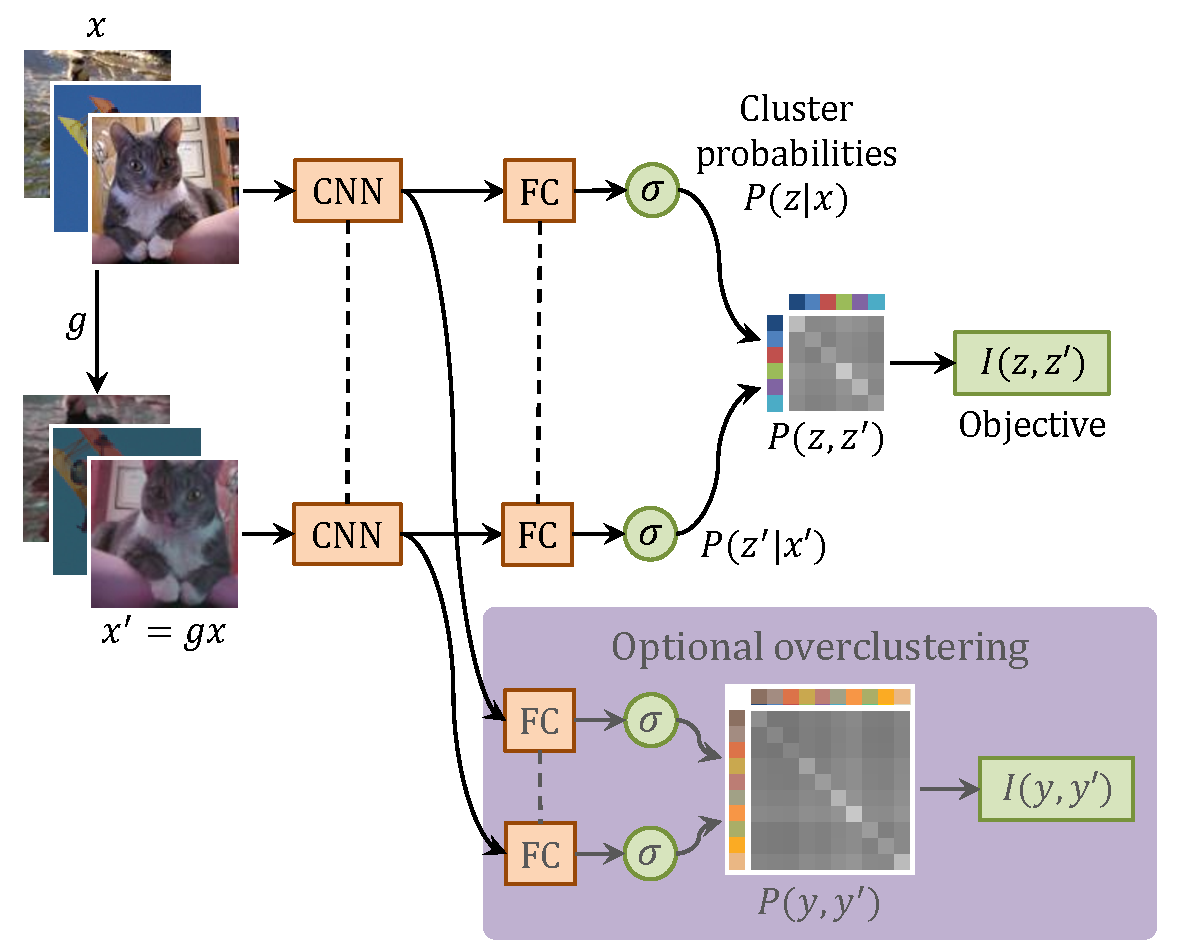
\includegraphics[width=0.95\columnwidth]{paper_imgs/overview1.pdf}
\caption{\label{f:overview}\methodnameshort for image clustering. Dashed line denotes shared parameters, $g$ is a random transformation, and $I$ denotes mutual information~(\cref{e:loss_expanded}).}
\end{figure}


\begin{figure*}
%\captionsetup{justification=centering}
\setlength\tabcolsep{2.2pt} % default value: 6pt

\begin{tabular}{c c c c c c}
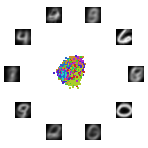
\includegraphics[height=0.16\textwidth]{experiments2_files/mnist_progression/726_run_1_colour_0_pointcloud_0.png} & 
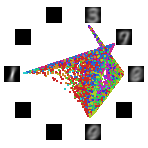
\includegraphics[height=0.16\textwidth]{experiments2_files/mnist_progression/726_run_1_colour_0_pointcloud_3.png} & 
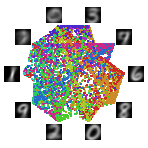
\includegraphics[height=0.16\textwidth]{experiments2_files/mnist_progression/726_run_1_colour_0_pointcloud_10.png} & 
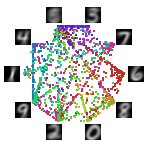
\includegraphics[height=0.16\textwidth]{experiments2_files/mnist_progression/726_run_1_colour_0_pointcloud_30.png} & 
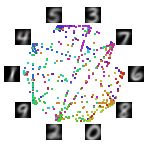
\includegraphics[height=0.16\textwidth]{experiments2_files/mnist_progression/726_run_1_colour_0_pointcloud_101.png} & 
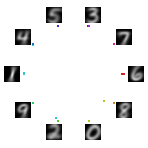
\includegraphics[height=0.16\textwidth]{experiments2_files/mnist_progression/726_run_1_colour_0_pointcloud_1000.png} 
\end{tabular}

\caption{\label{f:mnist_dots} Training with \methodnameshort on unlabelled MNIST in successive epochs from random initialisation (left). The network directly outputs cluster assignment probabilities for input images, and each is rendered as a coordinate by convex combination of 10 cluster vertices. There is no cherry-picking as the entire dataset is shown in every snapshot. Ground truth labelling (unseen by model) is given by colour. At each cluster the average image of its assignees is shown. With neither labels nor heuristics, the clusters discovered by \methodnameshort correspond perfectly to unique digits, with one-hot certain prediction (right).}
\end{figure*}


\paragraph{Co-clustering and mutual information.}

The use of information as a criterion to learn representations is not new. One of the earliest works to do so is by Becker and Hinton~\cite{becker1992self}.
More generally, learning from paired data has been explored in co-clustering~\cite{hartigan1972direct, dhillon2003information} and in other works~\cite{wang2010information} that build on the information bottleneck principle~\cite{friedman2001multivariate}.

Several recent papers have used information as a tool to train deep networks in particular.
IMSAT~\cite{hu2017learning} maximises mutual information between data and its representation and DeepINFOMAX~\cite{hjelm2018learning} maximizes information between spatially-preserved features and compact features.
However, IMSAT and DeepINFOMAX combine information with other criteria, whereas in our method information is the only criterion used.
Furthermore, both IMSAT and DeepINFOMAX compute mutual information over continuous random variables, which requires complex estimators~\cite{belghazi2018mine}, whereas \methodnameshort does so for discrete variables with simple and exact computations.
Finally, DeepINFOMAX considers the information $I(\bx, f(\bx))$ between the features $\bx$ and a deterministic function $f(\bx)$ of it, which is in principle the same as the entropy $H(\bx)$; in contrast, in \methodnameshort information does not trivially reduce to  entropy.

\paragraph{Semantic clustering versus intermediate representation learning.}
In semantic clustering, the learned function directly outputs discrete assignments for high level (i.e. semantic) clusters. Intermediate representation learners, on the other hand, produce continuous, distributed, high-dimensional representations that must be post-processed, for example by k-means, to obtain the discrete low-cardinality assignments required for unsupervised semantic clustering. The latter includes objectives such as generative autoencoder image reconstruction~\cite{vincent2010stacked},  triplets~\cite{schultz2004learning} and spatial-temporal order or context prediction~\cite{lee2017unsupervised,cruz2017deeppermnet,doersch2015unsupervised}, for example predicting patch proximity~\cite{isola2015learning}, solving jigsaw puzzles~\cite{noroozi2016unsupervised} and inpainting~\cite{pathak2016context}. Note it also includes a number of clustering methods (DeepCluster~\cite{caron2018deep}, exemplars~\cite{dosovitskiy2015discriminative}) where the clustering is only auxiliary; a clustering-style objective is used but does not produce groups with semantic correspondence. For example, DeepCluster~\cite{caron2018deep} is a state-of-the-art method for learning highly-transferable intermediate features using overclustering as a proxy task, but does not automatically find semantically meaningful clusters. As these methods use auxiliary objectives divorced from the semantic clustering objective, it is unsurprising that they perform worse than \methodnameshort~(\cref{s:experiments}), which directly optimises for it, training the network end-to-end with the final clusterer implicitly wrapped inside.




\paragraph{Optimising image-to-image distance.}

Many approaches to deep clustering, whether semantic or auxiliary, utilise a distance function between input images that approximates a given grouping criterion.
Agglomerative clustering~\cite{bautista2016cliquecnn} and partially ordered sets~\cite{bautista2017deep} of HOG features~\cite{dalal2005histograms} have been used to group images, and exemplars~\cite{dosovitskiy2015discriminative} define a group as a set of random transformations applied to a single image. Note the latter does not scale easily, in particular to image segmentation where a single $200\times 200$ image would call for 40k classes. DAC~\cite{chang2017deep}, JULE~\cite{yang2016joint}, DeepCluster~\cite{caron2018deep}, ADC~\cite{haeusser2018associative} and DEC~\cite{xie2016unsupervised} rely on the inherent visual consistency and disentangling properties~\cite{greff2015binding} of CNNs to produce cluster assignments, which are processed and reinforced in each iteration. 
The latter three are based on k-means style mechanisms to refine feature centroids, which is prone to degenerate solutions~\cite{caron2018deep} and thus needs explicit prevention mechanisms such as pre-training, cluster-reassignment or feature cleaning via PCA and whitening~\cite{xie2016unsupervised, caron2018deep}.

\begin{comment}
DAC is the only unsupervised clustering algorithm out of these that eschews k-means and agglomerative clustering for a different but similar clustering scheme, based on feature inner-products rather than distances.
DAC forms clusters gradually, in a self-paced manner, thus alleviating but not eliminating the risk of incurring degenerate solutions.
Furthermore, the nature of the optimisation, which reinforces bootstrapped class labels, creates a strong dependency on initialisation.

For unsupervised feature learning in general, i.e.\ where the training objective is not clustering, a large number of works explore using proxy learning tasks. 
There are two major directions:  generative tasks such as autoencoder image reconstruction~\cite{vincent2010stacked}, and spatial-temporal order or context prediction~\cite{lee2017unsupervised,cruz2017deeppermnet,doersch2015unsupervised}. The latter includes predicting patch proximity~\cite{isola2015learning}, solving jigsaw puzzles~\cite{noroozi2016unsupervised} and inpainting~\cite{pathak2016context}. 
In many cases they benefit from principled formulations that protect against degeneracy.
However, unlike the aforementioned clustering methods, the features learned by these methods need to be post-processed, for example using k-means, to cluster the data. 

\end{comment}

\paragraph{Invariance as a training objective.}

Optimising for function outputs to be persistent through spatio-temporal or non-material distortion is an idea shared by \methodnameshort with several works, including exemplars~\cite{dosovitskiy2015discriminative}, IMSAT~\cite{hu2017learning}, proximity prediction~\cite{isola2015learning}, the denoising objective of Tagger~\cite{greff2016tagger}, temporal slowness constraints~\cite{zou2012deep}, and optimising for features to be invariant to local image transformations~\cite{sohn2012learning,hui2013direct}.
More broadly, the problem of modelling data transformation has received significant attention in deep learning, one example being the transforming autoencoder~\cite{hinton2011transforming}.


% \section{Related work}\label{s:related}

% \paragraph{Co-clustering and mutual information.}

% The idea of learning a data representation by seeking the common parts of related observations is not new. 
% An early work is Becker and Hinton~\cite{becker1992self}, which maximises agreement between representations of 2D images to learn depth, using an objective corresponding to maximising mutual information between the input and the average of the data representations. 
% Co-learning has also been explored in the context of clustering by co-clustering methods, dating back to the pioneering work of Hartigan~\cite{hartigan72direct}. 
% Many information-theoretic variant of such approaches have been proposed, as discussed by~\cite{wang10information}, which are generally related to the information bottleneck principle~(\cite{friedman2001multivariate}). 

% A few works have employed mutual information in the context of unsupervised deep learning. IMSAT~\cite{hu2017learning} maximises mutual information between input data and their predicted discrete representations whilst encouraging the representations of augmented data points to be close to those of the original data points. 
% DeepINFOMAX~\cite{hjelm2018learning} maximises mutual information between spatially preserved features and compact features. There are some major differences with \methodnameshort. 
% Firstly, mutual information is used as an aid in these methods, as it increases the statistical predictivity between two random variables. 
% This contrasts with our method, where mutual information constitutes the loss applied directly to cluster assignments, meaning it is used as a clustering objective. 
% Secondly, both IMSAT and DeepINFOMAX compute mutual information over continuous random variables, which calls for an integral and is not computationally tractable, so estimators~\cite{belghazi2018mine} are used. 
% Since \methodnameshort maximises mutual information between cluster assignments and the number of clusters is discrete, computation is exact and straightforward. 
% Finally, DeepINFOMAX employs mutual information between function inputs and outputs, i.e. $I(x, f(x))$, but the conditional entropy component of mutual information $H(f(x) | x)$ is 0 when $f$ is deterministic, making the maximisation less meaningful. 
% In contrast \methodnameshort maximises mutual information between cluster assignments of separate images, i.e. $I(z, z')$ where $z$ and $z'$ are not functions of one other, making $H(z | z')$ a non-zero quantity that contributes to the optimisation as it can be minimised.

% \paragraph{Optimising image-to-image distance for clustering.}
% Many works for on unsupervised deep clustering involve establishing a scheme for estimating the semantic distance between input images, before training a function to learn this scheme. 
% CliqueCNN~\cite{bautista2016cliquecnn} trains a network to discriminate between cliques that are determined by applying agglomerative clustering on image features such as HOG~\cite{dalal2005histograms}. 
% In Exemplar CNNs~\cite{dosovitskiy2016discriminative}, each image and a its set of random transformations is considered a class, and a function is trained to discriminate between these surrogate classes. Like \methodnameshort, this method uses random transformations as a proxy for obtaining images with low semantic distance in the absence of label information. 
% Requiring one class per input image has a large memory footprint which makes Exemplar CNNs infeasible for segmentation (where patches are clustered instead of images, so a single 200x200 image would call for 40k classes). 

% \begin{figure}[t]
\centering
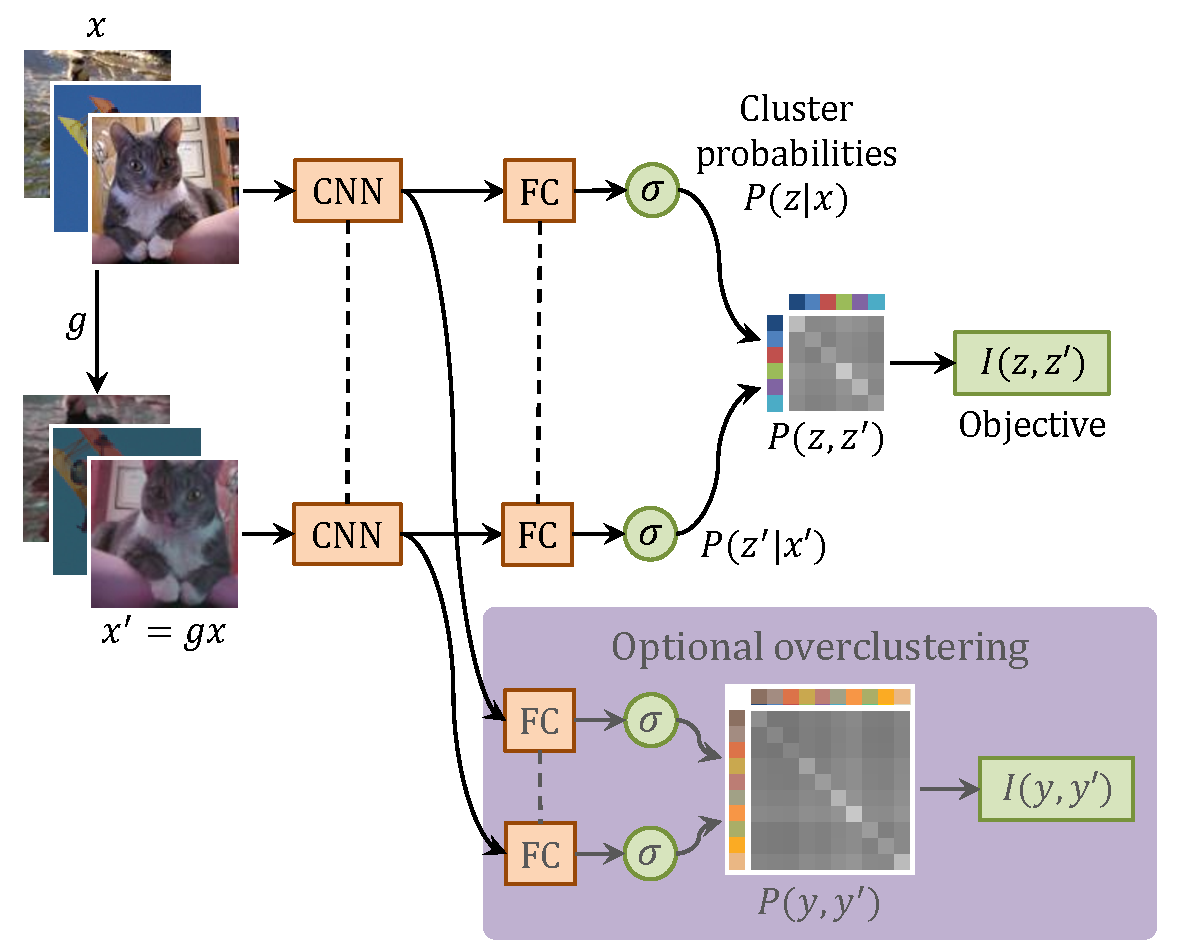
\includegraphics[width=0.95\columnwidth]{paper_imgs/overview1.pdf}
\caption{\label{f:overview}\methodnameshort for image clustering. Dashed line denotes shared parameters, $g$ is a random transformation, and $I$ denotes mutual information~(\cref{e:loss_expanded}).}
\end{figure}


% DAC~\cite{chang2017deep}, JULE~\cite{yang2016joint}, DeepCluster~\cite{caron2018deep}, Associative Deep Clustering~\cite{haeusser18associative} and DEC~\cite{xie2016unsupervised} all rely on the inherent visual consistency and disentangling properties~\cite{greff2015binding} of CNNs to produce meaningful cluster assignments, which are processed and reinforced in each iteration. 
% The latter three are based on using k-means to refine deep feature vectors, a mechanism which is prone to degenerate solutions~\cite{caron2018deep} and thus needs explicit prevention mechanisms such as pre-training, cluster-reassignment or feature cleaning via PCA and whitening ~\cite{xie2016unsupervised, caron2018deep}. 

% DAC is the only unsupervised clustering algorithm out of these that eschews k-means whilst training a network to directly produce cluster assignments, as \methodnameshort does. 
% A network is trained to produce cluster assignment probability distributions for each sample that are used as high level feature descriptors, and the dot product of different descriptors is treated as a proxy for inter-sample semantic distance (instead of Euclidian distance, which is used in the k-means based clusterers). 
% Training proceeds by maximising the dot product of close sample pairs, thus encouraging them to be assigned to the same cluster, whilst minimising the dot product for far pairs. 
% The nature of the optimisation means there is a strong dependency on initialisation and lack of protection against degenerate solutions such as clusters disappearing. 

% \paragraph{Proxy tasks for unsupervised feature learning.}
% For unsupervised feature learning in general, i.e. where the training objective is not clustering, a large number of works explore using proxy learning tasks. 
% There are two major camps:  generative tasks such as autoencoder image reconstruction~\cite{vincent2010stacked}, and spatial-temporal order or context prediction~\cite{lee2017unsupervised,cruz2017deeppermnet,doersch2015unsupervised}. The latter includes predicting patch proximity~\cite{isola2015learning}, solving jigsaw puzzles~(\cite{noroozi2016unsupervised}) and inpainting~(\cite{pathak2016context}). 
% In many cases they benefit from principled formulations that protect against degeneracy.
% However, unlike the aforementioned clustering methods, learned representations from these tasks constitute fine-grained continuous features rather than coarse cluster assignments, and thus must be post-processed, either by unsupervised clustering such as k-means or with label information via SVMs or fine-tuning, in order to produce semantic clusters.

% \paragraph{Invariance as a training objective.}
% Training for function outputs to be persistent through spatio-temporal distortion, noise distortion, or random transforms is an idea shared by \methodnameshort and several mentioned works, including Exemplar CNNs~\cite{dosovitskiy2016discriminative}, IMSAT~\cite{hu2017learning} and proximity prediction~\cite{isola2015learning}.
% It is also seen in Tagger~\cite{greff2016tagger}, which trains a function to denoise its input using several clusters to distribute the representation,~\cite{zou2012deep} which enforces a temporal slowness constraint on learned features, and~\cite{sohn2012learning,hui2013direct} which train for features invariant to local image transformations.



\vspace{-0.09in}
\section{Model}
\label{sec:model}

Our non-parametric approach to solving one-shot learning is based on two components which we describe in the following subsections. First, our model architecture follows recent advances in neural networks augmented with memory (as discussed in Section~\ref{sec:relwork}). Given a (small) support set $S$, our model defines a function $c_S$ (or classifier) for each $S$, i.e. a mapping $S \rightarrow c_S(.)$. Second, we employ a training strategy which is tailored for one-shot learning from the support set $S$.

\vspace{-0.09in}
\subsection{Model Architecture}

\begin{figure}[t]
\centering
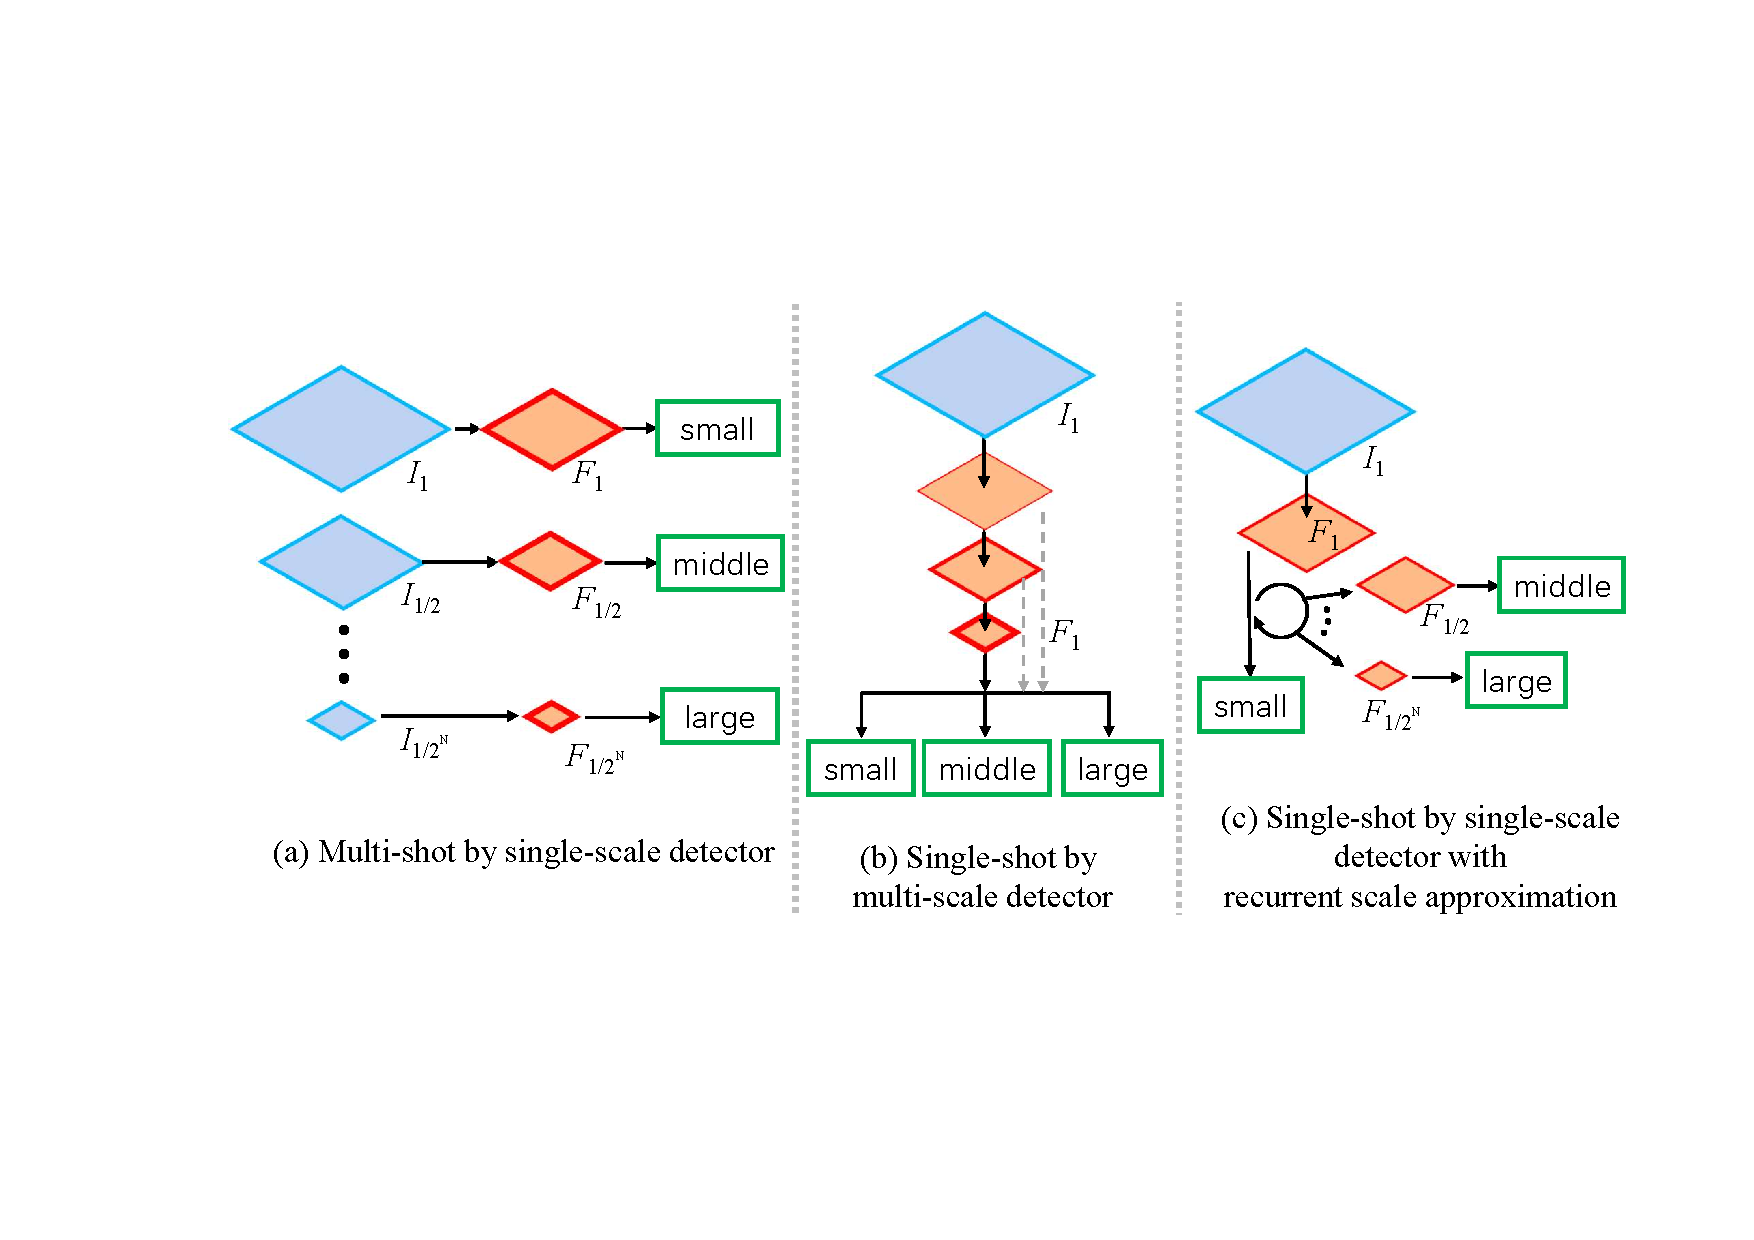
\includegraphics[width=.8\textwidth]{fig1}
\caption{\label{fig:arch}Matching Networks architecture}
\end{figure}

In recent years, many groups have investigated ways to augment neural network architectures with external memories and other components that make them more ``computer-like''. We draw inspiration from models such as sequence to sequence (seq2seq) with attention \cite{montreal}, memory networks \cite{memnets} and pointer networks \cite{ptrnets}.

In all these models, a neural attention mechanism, often fully differentiable, is defined to access (or read) a memory matrix which stores useful information to solve the task at hand. Typical uses of this include machine translation, speech recognition, or question answering. More generally, these architectures model $P(B|A)$ where $A$ and/or $B$ can be a sequence (like in seq2seq models), or, more interestingly for us, a set \cite{vinyals2015order}.

Our contribution is to cast the problem of one-shot learning within the set-to-set framework \cite{vinyals2015order}.
The key point is that when trained, Matching Networks are able to produce sensible test labels for unobserved classes \emph{without any changes to the network}.
More precisely, we wish to map from a (small) support set of $k$ examples of image-label pairs $S = \{(x_i, y_i)\}_{i=1}^k$ to a classifier $c_S(\hat{x})$ which, given a test example $\hat{x}$, defines a probability distribution over outputs $\hat{y}$.
We define the mapping $S\rightarrow c_S(\hat{x})$ to be $P(\hat{y} | \hat{x}, S)$ where $P$ is parameterised by a neural network. 
Thus, when given a new support set of examples $S'$ from which to one-shot learn, we simply use the parametric neural network defined by $P$ to make predictions about the appropriate label $\hat{y}$ for each test example $\hat{x}$: $P(\hat{y}|\hat{x}, S')$.
In general, our predicted output class for a given input unseen example $\hat{x}$ and a support set $S$ becomes $\arg\max_y P(y |\hat{x}, S)$.

Our model in its simplest form computes $\hat{y}$ as follows:

\begin{equation}
\hat{y} = \sum_{i=1}^{k} a(\hat{x},x_i) y_i
\label{eq:nn}
\end{equation}
where $x_i, y_i$ are the samples and labels from the support set $S=\{(x_i,y_i)\}_{i=1}^k$, and $a$ is an attention mechanism which we discuss below.
Note that eq.~\ref{eq:nn} essentially describes the output for a new class as a linear combination of the labels in the support set.
Where the attention mechanism $a$ is a kernel on $X\times X$, then \eqref{eq:nn} is akin to a kernel density estimator.
Where the attention mechanism is zero for the $b$ furthest $x_i$ from $\hat{x}$ according to some distance metric and an appropriate constant otherwise, then
\eqref{eq:nn} is equivalent to `$k-b$'-nearest neighbours (although this requires an extension to the attention mechanism that we describe in Section~\ref{sec:fce}).
Thus \eqref{eq:nn} subsumes both KDE and kNN methods.
Another view of \eqref{eq:nn} is where $a$ acts as an attention mechanism and the $y_i$ act as memories bound to the corresponding $x_i$.
In this case we can understand this as a particular kind of associative memory where, given an input, we ``point'' to the corresponding example in the support set, retrieving its label.
However, unlike other attentional memory mechanisms \cite{montreal}, \eqref{eq:nn} is non-parametric in nature: as the support set size grows, so does
the memory used.
Hence the functional form defined by the classifier $c_S(\hat{x})$ is very flexible and can adapt easily to any new support set.

\subsubsection{The Attention Kernel}
Equation~\ref{eq:nn} relies on choosing $a(.,.)$, the attention mechanism, which fully specifies the classifier. The simplest form that this takes (and which has very tight relationships with common attention models and kernel functions) is to use the softmax over the cosine distance $c$, i.e., 
$a(\hat{x},x_i) = e^{c(f(\hat{x}),g(x_i))} / \sum_{j=1}^k e^{c(f(\hat{x}),g(x_j))}$
with embedding functions $f$ and $g$ being appropriate neural networks (potentially with $f=g$) to embed $\hat{x}$ and $x_i$.
In our experiments we shall see examples where $f$ and $g$ are parameterised variously as deep convolutional networks for image tasks (as in VGG\cite{simonyan2014very} or Inception\cite{szegedy2015going}) or a simple form word embedding for language tasks (see Section~\ref{sec:results}).

We note that, though related to metric learning, the classifier defined by Equation~\ref{eq:nn} is discriminative. For a given support set $S$ and sample to classify $\hat{x}$, it is enough for $\hat{x}$ to be sufficiently aligned with pairs $(x',y') \in S$ such that $y'=y$ and misaligned with the rest. This kind of loss is also related to methods such as Neighborhood Component Analysis (NCA) \cite{nca}, triplet loss \cite{hoffer2015deep} or large margin nearest neighbor \cite{weinberger2009distance}.

However, the objective that we are trying to optimize is precisely aligned with multi-way, one-shot classification, and thus we expect it to perform better than its counterparts.
Additionally, the loss is simple and differentiable so that one can find the optimal parameters in an ``end-to-end'' fashion.

\subsubsection{Full Context Embeddings}
\label{sec:fce}
The main novelty of our model lies in reinterpreting a well studied framework (neural networks with external memories) to do one-shot learning. Closely related to metric learning, the embedding functions $f$ and $g$ act as a lift to feature space $X$ to achieve maximum accuracy through the classification function described in eq.~\ref{eq:nn}.

Despite the fact that the classification strategy is fully conditioned on the whole support set through $P(.|\hat{x},S)$, the embeddings on which we apply the cosine similarity to ``attend'', ``point'' or simply compute the nearest neighbor are myopic in the sense that each element $x_i$ gets embedded by $g(x_i)$ independently of other elements in the support set $S$. Furthermore, $S$ should be able to modify how we embed the test image $\hat{x}$ through $f$.

We propose embedding the elements of the set through a function which takes as input the full set $S$ in addition to $x_i$, i.e. $g$ becomes $g(x_i, S)$. Thus, as a function of the whole support set $S$, $g$ can modify how to embed $x_i$. This could be useful when some element $x_j$ is very close to $x_i$, in which case it may be beneficial to change the function with which we embed $x_i$ -- some evidence of this is discussed in Section~\ref{sec:results}.
We use a bidirectional Long-Short Term Memory (LSTM) \cite{hochreiter} to encode $x_i$ in the context of the support set $S$, considered as a sequence (see appendix for a more precise definition). 

The second issue can be fixed via an LSTM with read-attention over the whole set $S$, whose inputs are equal to $x$:
\begin{equation*}
f(\hat{x},S) = \text{attLSTM}(f'(\hat{x}), g(S), K)
\end{equation*}
where $f'(\hat{x})$ are the features (e.g., derived from a CNN) which are input to the LSTM (constant at each time step). $K$ is the fixed number of unrolling steps of the LSTM, and $g(S)$ is the set over which we attend, embedded with $g$. This allows for the model to potentially ignore some elements in the support set $S$, and adds ``depth'' to the computation of attention (see appendix for more details).

\subsection{Training Strategy}

In the previous subsection we described Matching Networks which map a support set to a classification function, $S \rightarrow c(\hat{x})$. We achieve this via a modification of the set-to-set paradigm augmented with attention, with the resulting mapping being of the form $P_\theta(.|\hat{x},S)$, noting that $\theta$ are the parameters of the model (i.e. of the embedding functions $f$ and $g$ described previously).

The training procedure has to be chosen carefully so as to match inference at test time. Our model has to perform well with support sets $S'$ which contain classes never seen during training.

More specifically, let us define a task $T$ as distribution over possible label sets $L$. Typically we consider $T$ to uniformly weight all data sets of up to a few unique classes (e.g., 5), with a few examples per class (e.g., up to 5).
In this case, a label set $L$ sampled from a task $T$,  $L \sim T$, will typically have 5 to 25 examples.

To form an ``episode'' to compute gradients and update our model, we first sample $L$ from $T$ (e.g., $L$ could be the label set $\{cats,dogs\}$). We then use $L$ to sample the support set $S$ and a batch $B$ (i.e., both $S$ and $B$ are labelled examples of cats and dogs).
The Matching Net is then trained to minimise the error predicting the labels in the batch $B$ conditioned on the support set $S$.
This is a form of meta-learning since the training procedure explicitly learns to learn from a given support set to minimise a loss over a batch.
More precisely, the Matching Nets training objective is as follows:
\begin{equation}
\theta = \arg\max_\theta E_{L \sim T} \left[ E_{S \sim L, B \sim L}\left[\sum_{(x,y) \in B} \log P_\theta\left(y|x, S\right)\right]\right].
\label{eqn:objf}
\end{equation}
Training $\theta$ with eq.~\ref{eqn:objf} yields a model which works well when sampling $S' \sim T'$ from a different distribution of novel labels. Crucially, our model does not need any fine tuning on the classes it has never seen due to its non-parametric nature. Obviously, as $T'$ diverges far from the $T$ from which we sampled to learn $\theta$, the model will not work -- we belabor this point further in Section~\ref{sec:imagenet}.
\section{Experiments}
\label{sect:experiments}

% \begin{figure*}
%   \centering
%   \setlength{\tabcolsep}{0pt}
%   \setlength\figurewidth{0.05\textwidth}
%   \newcommand{\example}[1]{\raisebox{-.4\height}{\includegraphics[width=\figurewidth]{./figures/domains_examples/#1}}}
%   \begin{sc}
%   \begin{tabular}{r@{\hskip 1cm} ccccccccccc}
%     MNIST \cite{LeCun98} &
%     \example{mnist_0.png} &
%     \example{mnist_1.png} &
%     \example{mnist_2.png} &
%     \example{mnist_3.png} &
%     \example{mnist_4.png} &
%     \example{mnist_5.png} &
%     \example{mnist_6.png} &
%     \example{mnist_7.png} &
%     \example{mnist_8.png} &
%     \example{mnist_9.png} &
%     \example{mnist_10.png}\\
%     MNIST ($ | \Delta | $, BG) &
%     \example{mnisti_0.png} &
%     \example{mnisti_1.png} &
%     \example{mnisti_2.png} &
%     \example{mnisti_3.png} &
%     \example{mnisti_4.png} &
%     \example{mnisti_5.png} &
%     \example{mnisti_6.png} &
%     \example{mnisti_7.png} &
%     \example{mnisti_8.png} &
%     \example{mnisti_9.png} &
%     \example{mnisti_10.png}\\
%     Syn Numbers &
%     \example{syn_0.png} &
%     \example{syn_1.png} &
%     \example{syn_2.png} &
%     \example{syn_3.png} &
%     \example{syn_4.png} &
%     \example{syn_5.png} &
%     \example{syn_6.png} &
%     \example{syn_7.png} &
%     \example{syn_8.png} &
%     \example{syn_9.png} &
%     \example{syn_10.png}\\
%     SVHN \cite{Netzer11} &
%     \example{svhn_0.png} &
%     \example{svhn_1.png} &
%     \example{svhn_2.png} &
%     \example{svhn_3.png} &
%     \example{svhn_4.png} &
%     \example{svhn_5.png} &
%     \example{svhn_6.png} &
%     \example{svhn_7.png} &
%     \example{svhn_8.png} &
%     \example{svhn_9.png} &
%     \example{svhn_10.png}\\
%     Syn Signs &
%     \example{synsgn_11.png} &
%     \example{synsgn_1.png} &
%     \example{synsgn_2.png} &
%     \example{synsgn_3.png} &
%     \example{synsgn_4.png} &
%     \example{synsgn_5.png} &
%     \example{synsgn_12.png} &
%     \example{synsgn_7.png} &
%     \example{synsgn_8.png} &
%     \example{synsgn_9.png} &
%     \example{synsgn_10.png}\\
%     GTSRB \cite{Stallkamp12} &
%     \example{gtsrb_0.png} &
%     \example{gtsrb_1.png} &
%     \example{gtsrb_2.png} &
%     \example{gtsrb_3.png} &
%     \example{gtsrb_4.png} &
%     \example{gtsrb_5.png} &
%     \example{gtsrb_6.png} &
%     \example{gtsrb_7.png} &
%     \example{gtsrb_8.png} &
%     \example{gtsrb_9.png} &
%     \example{gtsrb_10.png}\\
%     % CIFAR-10 \cite{Krizhevsky09} &
%     % \example{cifar10_0.png} &
%     % \example{cifar10_1.png} &
%     % \example{cifar10_2.png} &
%     % \example{cifar10_3.png} &
%     % \example{cifar10_4.png} &
%     % \example{cifar10_5.png} &
%     % \example{cifar10_11.png} &
%     % \example{cifar10_7.png} &
%     % \example{cifar10_8.png} &
%     % \example{cifar10_9.png} &
%     % \example{cifar10_10.png}\\
%     % STL-10 \cite{Coates11} &
%     % \example{stl10_12.png} &
%     % \example{stl10_1.png} &
%     % \example{stl10_2.png} &
%     % \example{stl10_3.png} &
%     % \example{stl10_4.png} &
%     % \example{stl10_5.png} &
%     % \example{stl10_6.png} &
%     % \example{stl10_13.png} &
%     % \example{stl10_8.png} &
%     % \example{stl10_9.png} &
%     % \example{stl10_10.png}\\
%   \end{tabular}
%   \end{sc}
%   \vskip 2.5mm
%   \caption{\todo[What to do with this figure? Add Office? Remove?]Random samples from the datasets used in the experiments. See \sect{exper_quant} for details.}
%   \label{fig:exper_domains_examples}
% \end{figure*}

\begin{figure*}
  \centering
  \setlength{\tabcolsep}{0pt}
  \setlength\figurewidth{0.05\textwidth}
  \newcommand{\example}[1]{\raisebox{-.4\height}{\includegraphics[width=\figurewidth]{./figures/domains_examples/#1}}}
  \begin{sc}
  \begin{small}
  \begin{tabular}{r@{\hskip 0.5cm} ccc c@{\hskip 0.4cm} ccc c@{\hskip 0.4cm} ccc c@{\hskip 0.4cm} ccc}
    &
    \multicolumn{3}{c}{MNIST} & &
    \multicolumn{3}{c}{Syn Numbers} & &
    \multicolumn{3}{c}{SVHN} & &
    \multicolumn{3}{c}{Syn Signs}\\
    
    Source &
    \example{mnist_0.png} &
    \example{mnist_1.png} &
    \example{mnist_3.png} & &
    
    \example{syn_0.png} &
    \example{syn_1.png} &
    \example{syn_2.png} & &
    
    \example{svhn_3.png} &
    \example{svhn_4.png} &
    \example{svhn_5.png} & &
    
    \example{synsgn_3.png} &
    \example{synsgn_4.png} &
    \example{synsgn_5.png}\\
    
    Target &
    \example{mnisti_0.png} &
    \example{mnisti_1.png} &
    \example{mnisti_2.png} & &
    
    \example{svhn_0.png} &
    \example{svhn_1.png} &
    \example{svhn_2.png} & &
    
    \example{mnist_4.png} &
    \example{mnist_5.png} &
    \example{mnist_6.png} & &
    
    \example{gtsrb_2.png} &
    \example{gtsrb_3.png} &
    \example{gtsrb_4.png}\\
    
    &
    \multicolumn{3}{c}{\rule{0pt}{0.35cm} MNIST-M} & &
    \multicolumn{3}{c}{SVHN} & &
    \multicolumn{3}{c}{MNIST} & &
    \multicolumn{3}{c}{GTSRB}\\
  \end{tabular}
  \end{small}
  \end{sc}
  \caption{Examples of domain pairs used in the experiments. See \sect{exper_quant} for details.}
  \label{fig:exper_domains_examples}
\end{figure*}


\begin{table*}[t]
  \vskip 0.15in
  \begin{center}
    \begin{small}
      \begin{sc}
        \renewcommand{\arraystretch}{1.5}
        \begin{tabular}{l r | c c c c}
          \hline
          \multirow{2}{*}{Method} & {\scriptsize Source} & MNIST & Syn Numbers & SVHN & Syn Signs \\
          & {\scriptsize Target} & MNIST-M & SVHN & MNIST & GTSRB \\
          \hline
          \multicolumn{2}{l |}{Source only} & 
          $ .5749 $                      & $ .8665 $                      & $ .5919 $                      & $ .7400 $                      \\
          \multicolumn{2}{l |}{SA \cite{Fernando13}} & 
          $ .6078 \; (7.9\%) $           & $ .8672 \; (1.3\%) $           & $ .6157 \; (5.9\%) $           & $ .7635 \; (9.1\%) $           \\
          \multicolumn{2}{l |}{Proposed approach} & 
          $ \mathbf{.8149} \; (57.9\%) $ & $ \mathbf{.9048} \; (66.1\%) $ & $ \mathbf{.7107} \; (29.3\%) $ & $ \mathbf{.8866} \; (56.7\%) $ \\
          \multicolumn{2}{l |}{Train on target} & 
          $ .9891 $                      & $ .9244 $                      & $ .9951 $                      & $ .9987 $                      \\
          \hline
        \end{tabular}
      \end{sc}
    \end{small}
  \end{center}
    \caption{Classification accuracies for digit image classifications for different source and target domains. {\sc MNIST-M} corresponds to difference-blended digits over non-uniform background. The first row corresponds to the lower performance bound (i.e.\ if no adaptation is performed). The last row corresponds to training on the target domain data with known class labels (upper bound on the DA performance). For each of the two DA methods (ours and \cite{Fernando13}) we show how much of the gap between the lower and the upper bounds was covered (in brackets). For all five cases, our approach outperforms \cite{Fernando13} considerably, and covers a big portion of the gap.\vspace{-0mm} }
  \label{tab:results}
  \vskip -0.1in
\end{table*}

\begin{table*}[t]
  \vskip 0.15in
  \begin{center}
    \begin{small}
      \begin{sc}
        \renewcommand{\arraystretch}{1.5}
        \begin{tabular}{l r | c c c}
          \hline
          \multirow{2}{*}{Method} & {\scriptsize Source} & Amazon & DSLR & Webcam \\
          & {\scriptsize Target} & Webcam & Webcam & DSLR \\
          \hline
          \multicolumn{2}{l |}{GFK(PLS, PCA) \cite{Gong12}} & 
          $ .464 \pm .005 $ & $ .613 \pm .004 $ & $ .663 \pm .004 $\\ 
          \multicolumn{2}{l |}{SA \cite{Fernando13}} & 
          $ .450 $ & $ .648 $ & $ .699 $\\ 
          \multicolumn{2}{l |}{DA-NBNN \cite{Tommasi13}} & 
          $ .528 \pm .037 $ & $ .766 \pm .017 $ & $ .762 \pm .025 $\\ 
          \multicolumn{2}{l |}{DLID \cite{Chopra13}} & 
          $ .519 $ & $ .782 $ & $ .899 $\\
          \multicolumn{2}{l |}{DeCAF$_6$ Source Only \cite{Donahue14}} &
          $ .522 \pm .017 $ & $ .915 \pm .015 $ & --\\ 
          \multicolumn{2}{l |}{DaNN \cite{Ghifary14}} & 
          $ .536 \pm .002 $ & $ .712 \pm .000 $ & $ .835 \pm .000 $\\ 
          \multicolumn{2}{l |}{DDC \cite{Tzeng14}} & 
          $ .594 \pm .008 $ & $ .925 \pm .003 $ & $ .917 \pm .008 $\\ 
          \multicolumn{2}{l |}{Proposed Approach} & 
          $ \mathbf{ .673 \pm .017 } $ & $ \mathbf{ .940 \pm .008 } $ & $ \mathbf{ .937 \pm .010 } $\\
          \hline
        \end{tabular}
      \end{sc}
    \end{small}
  \end{center}
    \caption{Accuracy evaluation of different DA approaches on the standard {\sc Office} \cite{Saenko10} dataset. Our method (last row) outperforms competitors setting the new state-of-the-art.}
  \label{tab:results_office}
\end{table*}

% Other rows refer to the following algorithms (from top to bottom): Geodesic Flow Kernel \cite{Gong12}, Subspace Alignment \cite{Fernando13}, Naive Bayes Nearest Neighbor \cite{Tommasi13},  deep learning approach from \cite{Chopra13}, DeCAF$_6$-features described in \cite{Donahue14}, Domain Adaptive NNs \cite{Ghifary14}, Deep Domain Confusion \cite{Tzeng14}.

\def\X{{\mathbf X}}
\def\y{{\mathbf y}}

% \vspace{2mm}\noindent {\bf Datasets.}
% \label{sect:exper_datasets}

% In order to test our method in the setting of traffic signs classification we obtained~100,000 synthetic images ({\sc Syn~Signs}) simulating various photoshooting conditions. This dataset was used in conjunction with {\it The German Traffic Sign Recognition Benchmark} ({\sc GTSRB}) \cite{Stallkamp12}.

% Finally, we perform domain adaption for the {\sc CIFAR-10} and the {\sc STL-10} downsampled to the size of $ 32 \times 32 $. This pair is considerably different from the previously mentioned datasets as the intra-class variability here is higher.

We perform extensive evaluation of the proposed approach on a number of popular image datasets and their modifications. These include large-scale datasets of small images popular with deep learning methods, and the {\sc Office} datasets \cite{Saenko10}, which are a {\em de facto} standard for domain adaptation in computer vision, but have much fewer images.

\vspace{2mm}\noindent {\bf Baselines.} For the bulk of experiments the following baselines are evaluated. The \textbf{source-only} model is trained without consideration for target-domain data (no domain classifier branch included into the network). The \textbf{train-on-target} model is trained on the target domain with class labels revealed. This model serves as an upper bound on DA methods, assuming that target data are abundant and the shift between the domains is considerable. 

In addition, we compare our approach against the recently proposed unsupervised DA method based on \textbf{subspace alignment (SA)} \cite{Fernando13}, which is simple to setup and test on new datasets, but has also been shown to perform very well in experimental comparisons with other ``shallow'' DA methods. To boost the performance of this baseline, we pick its most important free parameter (the number of principal components) from the range $ \{ 2, \ldots, 60 \} $, so that the test performance on the target domain is maximized. To apply SA in our setting, we train a source-only model and then consider the activations of the last hidden layer in the label predictor (before the final linear classifier) as descriptors/features, and learn the mapping between the source and the target domains \cite{Fernando13}.

Since the SA baseline requires to train a new classifier after adapting the features, and in order to put all the compared settings on an equal footing, we retrain the last layer of the label predictor using a standard linear SVM~\cite{liblinear} for all four considered methods (including ours; the performance on the target domain remains approximately the same after the retraining). 

For the {\sc Office} dataset \cite{Saenko10}, we directly compare the performance of our full network (feature extractor and label predictor) against recent DA approaches using previously published results.

\vspace{2mm}\noindent {\bf CNN architectures.} In general, we compose feature extractor from two or three convolutional layers, picking their exact configurations from previous works. We give the exact architectures in \ref{sect:appendix_archs}.

For the domain adaptator we stick to the three fully connected layers ($x\rightarrow1024\rightarrow1024\rightarrow2$), except for {\sc MNIST} where we used a simpler ($x\rightarrow100\rightarrow2$) architecture to speed up the experiments.

For loss functions, we set $ L_y $ and $ L_d $ to be the logistic regression loss and the binomial cross-entropy respectively.

\vspace{2mm}\noindent {\bf CNN training procedure.}
The model is trained on $128$-sized batches. Images are preprocessed by the mean subtraction. A half of each batch is populated by the samples from the source domain (with known labels), the rest is comprised of the target domain (with unknown labels).

In order to suppress noisy signal from the domain classifier at the early stages of the training procedure instead of fixing the adaptation factor $ \lambda $, we gradually change it from $0$ to $1$ using the following schedule:
\begin{equation}
  \lambda_p = \frac{2}{1 + \exp(-\gamma \cdot p)} - 1,
\end{equation}
where $\gamma$ was set to $10$ in all experiments (the schedule was not optimized/tweaked). Further details on the CNN training can be found in \ref{sect:appendix_training}.

\vspace{2mm}\noindent {\bf Visualizations.}
We use t-SNE \cite{Maaten13} projection to visualize feature distributions at different points of the network, while color-coding the domains (\fig{exper_adapt_vis}). We observe strong correspondence between the success of the adaptation in terms of the classification accuracy for the target domain, and the overlap between the domain distributions in such visualizations.
 
\vspace{2mm}\noindent {\bf Choosing meta-parameters.} 
In general, good unsupervised DA methods should provide ways to set meta-parameters (such as $\lambda$, the learning rate, the momentum rate, the network architecture for our method) in an unsupervised way, i.e.\ without referring to labeled data in the target domain. %Here we would like to give few recommendations concerning this matter. First, as it was pointed out in \sect{theory} the domain classifier should not be significantly more complex than the label predictor. 
In our method, one can assess the performance of the whole system (and the effect of changing hyper-parameters) by observing the test error on the source domain {\em and} the domain classifier error. In general, we observed a good correspondence between the success of adaptation and these errors (adaptation is more successful when the source domain test error is low, while the domain classifier error is high).
In addition, the layer, where the the domain adaptator is attached can be picked by computing difference between means as suggested in \cite{Tzeng14}. 

% \begin{figure*}
%   \centering
%   {\sc MNIST $ \rightarrow $ MNIST ($ | \Delta | $, bg)}: top feature extractor layer
%   \setcounter{subfigure}{0}
%   \subfigure[Non-adapted]{%%
%     \scalebox{0.8}{%% Creator: Matplotlib, PGF backend
%%
%% To include the figure in your LaTeX document, write
%%   \input{<filename>.pgf}
%%
%% Make sure the required packages are loaded in your preamble
%%   \usepackage{pgf}
%%
%% Figures using additional raster images can only be included by \input if
%% they are in the same directory as the main LaTeX file. For loading figures
%% from other directories you can use the `import` package
%%   \usepackage{import}
%% and then include the figures with
%%   \import{<path to file>}{<filename>.pgf}
%%
%% Matplotlib used the following preamble
%%   \usepackage[utf8x]{inputenc}
%%   \usepackage[T1]{fontenc}
%%
\begingroup%
\makeatletter%
\begin{pgfpicture}%
\pgfpathrectangle{\pgfpointorigin}{\pgfqpoint{3.338520in}{2.040000in}}%
\pgfusepath{use as bounding box}%
\begin{pgfscope}%
\pgfsetbuttcap%
\pgfsetroundjoin%
\definecolor{currentfill}{rgb}{1.000000,1.000000,1.000000}%
\pgfsetfillcolor{currentfill}%
\pgfsetlinewidth{0.000000pt}%
\definecolor{currentstroke}{rgb}{1.000000,1.000000,1.000000}%
\pgfsetstrokecolor{currentstroke}%
\pgfsetdash{}{0pt}%
\pgfpathmoveto{\pgfqpoint{0.000000in}{-0.000000in}}%
\pgfpathlineto{\pgfqpoint{3.338520in}{-0.000000in}}%
\pgfpathlineto{\pgfqpoint{3.338520in}{2.040000in}}%
\pgfpathlineto{\pgfqpoint{0.000000in}{2.040000in}}%
\pgfpathclose%
\pgfusepath{fill}%
\end{pgfscope}%
\begin{pgfscope}%
\pgftext[at=\pgfqpoint{0.510000in}{0.348333in},left,bottom]{\pgfimage[interpolate=true,width=2.553333in,height=1.500000in]{./figures/adaptation_vis/pool2_mnist2inv_before-img0.png}}%
\end{pgfscope}%
\begin{pgfscope}%
\pgftext[at=\pgfqpoint{0.805000in}{0.383333in},left,bottom]{\pgfimage[interpolate=true,width=2.201667in,height=1.371667in]{./figures/adaptation_vis/pool2_mnist2inv_before-img1.png}}%
\end{pgfscope}%
\end{pgfpicture}%
\makeatother%
\endgroup%
}}%%
%   \subfigure[Adapted]{%%
%     \scalebox{0.8}{%% Creator: Matplotlib, PGF backend
%%
%% To include the figure in your LaTeX document, write
%%   \input{<filename>.pgf}
%%
%% Make sure the required packages are loaded in your preamble
%%   \usepackage{pgf}
%%
%% Figures using additional raster images can only be included by \input if
%% they are in the same directory as the main LaTeX file. For loading figures
%% from other directories you can use the `import` package
%%   \usepackage{import}
%% and then include the figures with
%%   \import{<path to file>}{<filename>.pgf}
%%
%% Matplotlib used the following preamble
%%   \usepackage[utf8x]{inputenc}
%%   \usepackage[T1]{fontenc}
%%
\begingroup%
\makeatletter%
\begin{pgfpicture}%
\pgfpathrectangle{\pgfpointorigin}{\pgfqpoint{3.340000in}{2.040000in}}%
\pgfusepath{use as bounding box}%
\begin{pgfscope}%
\pgfsetbuttcap%
\pgfsetroundjoin%
\definecolor{currentfill}{rgb}{1.000000,1.000000,1.000000}%
\pgfsetfillcolor{currentfill}%
\pgfsetlinewidth{0.000000pt}%
\definecolor{currentstroke}{rgb}{1.000000,1.000000,1.000000}%
\pgfsetstrokecolor{currentstroke}%
\pgfsetdash{}{0pt}%
\pgfpathmoveto{\pgfqpoint{0.000000in}{-0.000000in}}%
\pgfpathlineto{\pgfqpoint{3.340000in}{-0.000000in}}%
\pgfpathlineto{\pgfqpoint{3.340000in}{2.040000in}}%
\pgfpathlineto{\pgfqpoint{0.000000in}{2.040000in}}%
\pgfpathclose%
\pgfusepath{fill}%
\end{pgfscope}%
\begin{pgfscope}%
\pgftext[at=\pgfqpoint{0.518333in}{0.321667in},left,bottom]{\pgfimage[interpolate=true,width=2.565000in,height=1.550000in]{./figures/adaptation_vis/pool2_mnist2inv_after-img0.png}}%
\end{pgfscope}%
\begin{pgfscope}%
\pgftext[at=\pgfqpoint{0.518333in}{0.321667in},left,bottom]{\pgfimage[interpolate=true,width=2.565000in,height=1.553333in]{./figures/adaptation_vis/pool2_mnist2inv_after-img1.png}}%
\end{pgfscope}%
\end{pgfpicture}%
\makeatother%
\endgroup%
}}\\
%   \vspace{5mm}
%   {\sc Syn Numbers $ \rightarrow $ SVHN}: last hidden layer of the label predictor
%   \setcounter{subfigure}{0}
%   \subfigure[Non-adapted]{%%
%     \scalebox{0.8}{%% Creator: Matplotlib, PGF backend
%%
%% To include the figure in your LaTeX document, write
%%   \input{<filename>.pgf}
%%
%% Make sure the required packages are loaded in your preamble
%%   \usepackage{pgf}
%%
%% Figures using additional raster images can only be included by \input if
%% they are in the same directory as the main LaTeX file. For loading figures
%% from other directories you can use the `import` package
%%   \usepackage{import}
%% and then include the figures with
%%   \import{<path to file>}{<filename>.pgf}
%%
%% Matplotlib used the following preamble
%%   \usepackage[utf8x]{inputenc}
%%   \usepackage[T1]{fontenc}
%%
\begingroup%
\makeatletter%
\begin{pgfpicture}%
\pgfpathrectangle{\pgfpointorigin}{\pgfqpoint{3.340000in}{2.040000in}}%
\pgfusepath{use as bounding box}%
\begin{pgfscope}%
\pgfsetbuttcap%
\pgfsetroundjoin%
\definecolor{currentfill}{rgb}{1.000000,1.000000,1.000000}%
\pgfsetfillcolor{currentfill}%
\pgfsetlinewidth{0.000000pt}%
\definecolor{currentstroke}{rgb}{1.000000,1.000000,1.000000}%
\pgfsetstrokecolor{currentstroke}%
\pgfsetdash{}{0pt}%
\pgfpathmoveto{\pgfqpoint{0.000000in}{-0.000000in}}%
\pgfpathlineto{\pgfqpoint{3.340000in}{-0.000000in}}%
\pgfpathlineto{\pgfqpoint{3.340000in}{2.040000in}}%
\pgfpathlineto{\pgfqpoint{0.000000in}{2.040000in}}%
\pgfpathclose%
\pgfusepath{fill}%
\end{pgfscope}%
\begin{pgfscope}%
\pgftext[at=\pgfqpoint{0.491667in}{0.335000in},left,bottom]{\pgfimage[interpolate=true,width=2.618333in,height=1.531667in]{./figures/adaptation_vis/before-img0.png}}%
\end{pgfscope}%
\begin{pgfscope}%
\pgftext[at=\pgfqpoint{0.758333in}{0.331667in},left,bottom]{\pgfimage[interpolate=true,width=2.171667in,height=1.436667in]{./figures/adaptation_vis/before-img1.png}}%
\end{pgfscope}%
\begin{pgfscope}%
\pgfsetbuttcap%
\pgfsetroundjoin%
\definecolor{currentfill}{rgb}{0.000000,0.000000,1.000000}%
\pgfsetfillcolor{currentfill}%
\pgfsetfillopacity{0.300000}%
\pgfsetlinewidth{0.150562pt}%
\definecolor{currentstroke}{rgb}{0.000000,0.000000,0.000000}%
\pgfsetstrokecolor{currentstroke}%
\pgfsetstrokeopacity{0.300000}%
\pgfsetdash{}{0pt}%
\pgfpathmoveto{\pgfqpoint{2.521160in}{1.775861in}}%
\pgfpathcurveto{\pgfqpoint{2.525278in}{1.775861in}}{\pgfqpoint{2.529228in}{1.777497in}}{\pgfqpoint{2.532140in}{1.780409in}}%
\pgfpathcurveto{\pgfqpoint{2.535052in}{1.783321in}}{\pgfqpoint{2.536688in}{1.787271in}}{\pgfqpoint{2.536688in}{1.791389in}}%
\pgfpathcurveto{\pgfqpoint{2.536688in}{1.795507in}}{\pgfqpoint{2.535052in}{1.799457in}}{\pgfqpoint{2.532140in}{1.802369in}}%
\pgfpathcurveto{\pgfqpoint{2.529228in}{1.805281in}}{\pgfqpoint{2.525278in}{1.806917in}}{\pgfqpoint{2.521160in}{1.806917in}}%
\pgfpathcurveto{\pgfqpoint{2.517042in}{1.806917in}}{\pgfqpoint{2.513092in}{1.805281in}}{\pgfqpoint{2.510180in}{1.802369in}}%
\pgfpathcurveto{\pgfqpoint{2.507268in}{1.799457in}}{\pgfqpoint{2.505631in}{1.795507in}}{\pgfqpoint{2.505631in}{1.791389in}}%
\pgfpathcurveto{\pgfqpoint{2.505631in}{1.787271in}}{\pgfqpoint{2.507268in}{1.783321in}}{\pgfqpoint{2.510180in}{1.780409in}}%
\pgfpathcurveto{\pgfqpoint{2.513092in}{1.777497in}}{\pgfqpoint{2.517042in}{1.775861in}}{\pgfqpoint{2.521160in}{1.775861in}}%
\pgfpathclose%
\pgfusepath{stroke,fill}%
\end{pgfscope}%
\begin{pgfscope}%
\pgfsetbuttcap%
\pgfsetroundjoin%
\definecolor{currentfill}{rgb}{0.000000,0.000000,1.000000}%
\pgfsetfillcolor{currentfill}%
\pgfsetfillopacity{0.300000}%
\pgfsetlinewidth{0.150562pt}%
\definecolor{currentstroke}{rgb}{0.000000,0.000000,0.000000}%
\pgfsetstrokecolor{currentstroke}%
\pgfsetstrokeopacity{0.300000}%
\pgfsetdash{}{0pt}%
\pgfpathmoveto{\pgfqpoint{2.598938in}{1.785583in}}%
\pgfpathcurveto{\pgfqpoint{2.603056in}{1.785583in}}{\pgfqpoint{2.607006in}{1.787219in}}{\pgfqpoint{2.609918in}{1.790131in}}%
\pgfpathcurveto{\pgfqpoint{2.612830in}{1.793043in}}{\pgfqpoint{2.614466in}{1.796993in}}{\pgfqpoint{2.614466in}{1.801111in}}%
\pgfpathcurveto{\pgfqpoint{2.614466in}{1.805229in}}{\pgfqpoint{2.612830in}{1.809179in}}{\pgfqpoint{2.609918in}{1.812091in}}%
\pgfpathcurveto{\pgfqpoint{2.607006in}{1.815003in}}{\pgfqpoint{2.603056in}{1.816639in}}{\pgfqpoint{2.598938in}{1.816639in}}%
\pgfpathcurveto{\pgfqpoint{2.594819in}{1.816639in}}{\pgfqpoint{2.590869in}{1.815003in}}{\pgfqpoint{2.587957in}{1.812091in}}%
\pgfpathcurveto{\pgfqpoint{2.585045in}{1.809179in}}{\pgfqpoint{2.583409in}{1.805229in}}{\pgfqpoint{2.583409in}{1.801111in}}%
\pgfpathcurveto{\pgfqpoint{2.583409in}{1.796993in}}{\pgfqpoint{2.585045in}{1.793043in}}{\pgfqpoint{2.587957in}{1.790131in}}%
\pgfpathcurveto{\pgfqpoint{2.590869in}{1.787219in}}{\pgfqpoint{2.594819in}{1.785583in}}{\pgfqpoint{2.598938in}{1.785583in}}%
\pgfpathclose%
\pgfusepath{stroke,fill}%
\end{pgfscope}%
\begin{pgfscope}%
\pgfsetbuttcap%
\pgfsetroundjoin%
\definecolor{currentfill}{rgb}{0.000000,0.000000,1.000000}%
\pgfsetfillcolor{currentfill}%
\pgfsetfillopacity{0.300000}%
\pgfsetlinewidth{0.150562pt}%
\definecolor{currentstroke}{rgb}{0.000000,0.000000,0.000000}%
\pgfsetstrokecolor{currentstroke}%
\pgfsetstrokeopacity{0.300000}%
\pgfsetdash{}{0pt}%
\pgfpathmoveto{\pgfqpoint{2.676715in}{1.771000in}}%
\pgfpathcurveto{\pgfqpoint{2.680833in}{1.771000in}}{\pgfqpoint{2.684783in}{1.772636in}}{\pgfqpoint{2.687695in}{1.775548in}}%
\pgfpathcurveto{\pgfqpoint{2.690607in}{1.778460in}}{\pgfqpoint{2.692244in}{1.782410in}}{\pgfqpoint{2.692244in}{1.786528in}}%
\pgfpathcurveto{\pgfqpoint{2.692244in}{1.790646in}}{\pgfqpoint{2.690607in}{1.794596in}}{\pgfqpoint{2.687695in}{1.797508in}}%
\pgfpathcurveto{\pgfqpoint{2.684783in}{1.800420in}}{\pgfqpoint{2.680833in}{1.802056in}}{\pgfqpoint{2.676715in}{1.802056in}}%
\pgfpathcurveto{\pgfqpoint{2.672597in}{1.802056in}}{\pgfqpoint{2.668647in}{1.800420in}}{\pgfqpoint{2.665735in}{1.797508in}}%
\pgfpathcurveto{\pgfqpoint{2.662823in}{1.794596in}}{\pgfqpoint{2.661187in}{1.790646in}}{\pgfqpoint{2.661187in}{1.786528in}}%
\pgfpathcurveto{\pgfqpoint{2.661187in}{1.782410in}}{\pgfqpoint{2.662823in}{1.778460in}}{\pgfqpoint{2.665735in}{1.775548in}}%
\pgfpathcurveto{\pgfqpoint{2.668647in}{1.772636in}}{\pgfqpoint{2.672597in}{1.771000in}}{\pgfqpoint{2.676715in}{1.771000in}}%
\pgfpathclose%
\pgfusepath{stroke,fill}%
\end{pgfscope}%
\begin{pgfscope}%
\pgftext[x=2.798938in,y=1.762222in,left,base]{{\rmfamily\fontsize{8.000000}{9.600000}\selectfont Source}}%
\end{pgfscope}%
\begin{pgfscope}%
\pgfsetbuttcap%
\pgfsetroundjoin%
\definecolor{currentfill}{rgb}{1.000000,0.000000,0.000000}%
\pgfsetfillcolor{currentfill}%
\pgfsetfillopacity{0.300000}%
\pgfsetlinewidth{0.150562pt}%
\definecolor{currentstroke}{rgb}{0.000000,0.000000,0.000000}%
\pgfsetstrokecolor{currentstroke}%
\pgfsetstrokeopacity{0.300000}%
\pgfsetdash{}{0pt}%
\pgfpathmoveto{\pgfqpoint{2.521160in}{1.620928in}}%
\pgfpathcurveto{\pgfqpoint{2.525278in}{1.620928in}}{\pgfqpoint{2.529228in}{1.622564in}}{\pgfqpoint{2.532140in}{1.625476in}}%
\pgfpathcurveto{\pgfqpoint{2.535052in}{1.628388in}}{\pgfqpoint{2.536688in}{1.632338in}}{\pgfqpoint{2.536688in}{1.636456in}}%
\pgfpathcurveto{\pgfqpoint{2.536688in}{1.640574in}}{\pgfqpoint{2.535052in}{1.644524in}}{\pgfqpoint{2.532140in}{1.647436in}}%
\pgfpathcurveto{\pgfqpoint{2.529228in}{1.650348in}}{\pgfqpoint{2.525278in}{1.651984in}}{\pgfqpoint{2.521160in}{1.651984in}}%
\pgfpathcurveto{\pgfqpoint{2.517042in}{1.651984in}}{\pgfqpoint{2.513092in}{1.650348in}}{\pgfqpoint{2.510180in}{1.647436in}}%
\pgfpathcurveto{\pgfqpoint{2.507268in}{1.644524in}}{\pgfqpoint{2.505631in}{1.640574in}}{\pgfqpoint{2.505631in}{1.636456in}}%
\pgfpathcurveto{\pgfqpoint{2.505631in}{1.632338in}}{\pgfqpoint{2.507268in}{1.628388in}}{\pgfqpoint{2.510180in}{1.625476in}}%
\pgfpathcurveto{\pgfqpoint{2.513092in}{1.622564in}}{\pgfqpoint{2.517042in}{1.620928in}}{\pgfqpoint{2.521160in}{1.620928in}}%
\pgfpathclose%
\pgfusepath{stroke,fill}%
\end{pgfscope}%
\begin{pgfscope}%
\pgfsetbuttcap%
\pgfsetroundjoin%
\definecolor{currentfill}{rgb}{1.000000,0.000000,0.000000}%
\pgfsetfillcolor{currentfill}%
\pgfsetfillopacity{0.300000}%
\pgfsetlinewidth{0.150562pt}%
\definecolor{currentstroke}{rgb}{0.000000,0.000000,0.000000}%
\pgfsetstrokecolor{currentstroke}%
\pgfsetstrokeopacity{0.300000}%
\pgfsetdash{}{0pt}%
\pgfpathmoveto{\pgfqpoint{2.598938in}{1.630650in}}%
\pgfpathcurveto{\pgfqpoint{2.603056in}{1.630650in}}{\pgfqpoint{2.607006in}{1.632286in}}{\pgfqpoint{2.609918in}{1.635198in}}%
\pgfpathcurveto{\pgfqpoint{2.612830in}{1.638110in}}{\pgfqpoint{2.614466in}{1.642060in}}{\pgfqpoint{2.614466in}{1.646178in}}%
\pgfpathcurveto{\pgfqpoint{2.614466in}{1.650296in}}{\pgfqpoint{2.612830in}{1.654246in}}{\pgfqpoint{2.609918in}{1.657158in}}%
\pgfpathcurveto{\pgfqpoint{2.607006in}{1.660070in}}{\pgfqpoint{2.603056in}{1.661706in}}{\pgfqpoint{2.598938in}{1.661706in}}%
\pgfpathcurveto{\pgfqpoint{2.594819in}{1.661706in}}{\pgfqpoint{2.590869in}{1.660070in}}{\pgfqpoint{2.587957in}{1.657158in}}%
\pgfpathcurveto{\pgfqpoint{2.585045in}{1.654246in}}{\pgfqpoint{2.583409in}{1.650296in}}{\pgfqpoint{2.583409in}{1.646178in}}%
\pgfpathcurveto{\pgfqpoint{2.583409in}{1.642060in}}{\pgfqpoint{2.585045in}{1.638110in}}{\pgfqpoint{2.587957in}{1.635198in}}%
\pgfpathcurveto{\pgfqpoint{2.590869in}{1.632286in}}{\pgfqpoint{2.594819in}{1.630650in}}{\pgfqpoint{2.598938in}{1.630650in}}%
\pgfpathclose%
\pgfusepath{stroke,fill}%
\end{pgfscope}%
\begin{pgfscope}%
\pgfsetbuttcap%
\pgfsetroundjoin%
\definecolor{currentfill}{rgb}{1.000000,0.000000,0.000000}%
\pgfsetfillcolor{currentfill}%
\pgfsetfillopacity{0.300000}%
\pgfsetlinewidth{0.150562pt}%
\definecolor{currentstroke}{rgb}{0.000000,0.000000,0.000000}%
\pgfsetstrokecolor{currentstroke}%
\pgfsetstrokeopacity{0.300000}%
\pgfsetdash{}{0pt}%
\pgfpathmoveto{\pgfqpoint{2.676715in}{1.616066in}}%
\pgfpathcurveto{\pgfqpoint{2.680833in}{1.616066in}}{\pgfqpoint{2.684783in}{1.617703in}}{\pgfqpoint{2.687695in}{1.620615in}}%
\pgfpathcurveto{\pgfqpoint{2.690607in}{1.623527in}}{\pgfqpoint{2.692244in}{1.627477in}}{\pgfqpoint{2.692244in}{1.631595in}}%
\pgfpathcurveto{\pgfqpoint{2.692244in}{1.635713in}}{\pgfqpoint{2.690607in}{1.639663in}}{\pgfqpoint{2.687695in}{1.642575in}}%
\pgfpathcurveto{\pgfqpoint{2.684783in}{1.645487in}}{\pgfqpoint{2.680833in}{1.647123in}}{\pgfqpoint{2.676715in}{1.647123in}}%
\pgfpathcurveto{\pgfqpoint{2.672597in}{1.647123in}}{\pgfqpoint{2.668647in}{1.645487in}}{\pgfqpoint{2.665735in}{1.642575in}}%
\pgfpathcurveto{\pgfqpoint{2.662823in}{1.639663in}}{\pgfqpoint{2.661187in}{1.635713in}}{\pgfqpoint{2.661187in}{1.631595in}}%
\pgfpathcurveto{\pgfqpoint{2.661187in}{1.627477in}}{\pgfqpoint{2.662823in}{1.623527in}}{\pgfqpoint{2.665735in}{1.620615in}}%
\pgfpathcurveto{\pgfqpoint{2.668647in}{1.617703in}}{\pgfqpoint{2.672597in}{1.616066in}}{\pgfqpoint{2.676715in}{1.616066in}}%
\pgfpathclose%
\pgfusepath{stroke,fill}%
\end{pgfscope}%
\begin{pgfscope}%
\pgftext[x=2.798938in,y=1.607289in,left,base]{{\rmfamily\fontsize{8.000000}{9.600000}\selectfont Target}}%
\end{pgfscope}%
\end{pgfpicture}%
\makeatother%
\endgroup%
}}%%
%   \subfigure[Adapted]{%%
%     \scalebox{0.8}{%% Creator: Matplotlib, PGF backend
%%
%% To include the figure in your LaTeX document, write
%%   \input{<filename>.pgf}
%%
%% Make sure the required packages are loaded in your preamble
%%   \usepackage{pgf}
%%
%% Figures using additional raster images can only be included by \input if
%% they are in the same directory as the main LaTeX file. For loading figures
%% from other directories you can use the `import` package
%%   \usepackage{import}
%% and then include the figures with
%%   \import{<path to file>}{<filename>.pgf}
%%
%% Matplotlib used the following preamble
%%   \usepackage[utf8x]{inputenc}
%%   \usepackage[T1]{fontenc}
%%
\begingroup%
\makeatletter%
\begin{pgfpicture}%
\pgfpathrectangle{\pgfpointorigin}{\pgfqpoint{3.340000in}{2.040000in}}%
\pgfusepath{use as bounding box}%
\begin{pgfscope}%
\pgfsetbuttcap%
\pgfsetroundjoin%
\definecolor{currentfill}{rgb}{1.000000,1.000000,1.000000}%
\pgfsetfillcolor{currentfill}%
\pgfsetlinewidth{0.000000pt}%
\definecolor{currentstroke}{rgb}{1.000000,1.000000,1.000000}%
\pgfsetstrokecolor{currentstroke}%
\pgfsetdash{}{0pt}%
\pgfpathmoveto{\pgfqpoint{0.000000in}{-0.000000in}}%
\pgfpathlineto{\pgfqpoint{3.340000in}{-0.000000in}}%
\pgfpathlineto{\pgfqpoint{3.340000in}{2.040000in}}%
\pgfpathlineto{\pgfqpoint{0.000000in}{2.040000in}}%
\pgfpathclose%
\pgfusepath{fill}%
\end{pgfscope}%
\begin{pgfscope}%
\pgftext[at=\pgfqpoint{0.501667in}{0.330000in},left,bottom]{\pgfimage[interpolate=true,width=2.600000in,height=1.540000in]{./figures/adaptation_vis/after-img0.png}}%
\end{pgfscope}%
\begin{pgfscope}%
\pgftext[at=\pgfqpoint{0.500000in}{0.320000in},left,bottom]{\pgfimage[interpolate=true,width=2.585000in,height=1.556667in]{./figures/adaptation_vis/after-img1.png}}%
\end{pgfscope}%
\begin{pgfscope}%
\pgfsetbuttcap%
\pgfsetroundjoin%
\definecolor{currentfill}{rgb}{0.000000,0.000000,1.000000}%
\pgfsetfillcolor{currentfill}%
\pgfsetfillopacity{0.300000}%
\pgfsetlinewidth{0.150562pt}%
\definecolor{currentstroke}{rgb}{0.000000,0.000000,0.000000}%
\pgfsetstrokecolor{currentstroke}%
\pgfsetstrokeopacity{0.300000}%
\pgfsetdash{}{0pt}%
\pgfpathmoveto{\pgfqpoint{2.521160in}{1.775861in}}%
\pgfpathcurveto{\pgfqpoint{2.525278in}{1.775861in}}{\pgfqpoint{2.529228in}{1.777497in}}{\pgfqpoint{2.532140in}{1.780409in}}%
\pgfpathcurveto{\pgfqpoint{2.535052in}{1.783321in}}{\pgfqpoint{2.536688in}{1.787271in}}{\pgfqpoint{2.536688in}{1.791389in}}%
\pgfpathcurveto{\pgfqpoint{2.536688in}{1.795507in}}{\pgfqpoint{2.535052in}{1.799457in}}{\pgfqpoint{2.532140in}{1.802369in}}%
\pgfpathcurveto{\pgfqpoint{2.529228in}{1.805281in}}{\pgfqpoint{2.525278in}{1.806917in}}{\pgfqpoint{2.521160in}{1.806917in}}%
\pgfpathcurveto{\pgfqpoint{2.517042in}{1.806917in}}{\pgfqpoint{2.513092in}{1.805281in}}{\pgfqpoint{2.510180in}{1.802369in}}%
\pgfpathcurveto{\pgfqpoint{2.507268in}{1.799457in}}{\pgfqpoint{2.505631in}{1.795507in}}{\pgfqpoint{2.505631in}{1.791389in}}%
\pgfpathcurveto{\pgfqpoint{2.505631in}{1.787271in}}{\pgfqpoint{2.507268in}{1.783321in}}{\pgfqpoint{2.510180in}{1.780409in}}%
\pgfpathcurveto{\pgfqpoint{2.513092in}{1.777497in}}{\pgfqpoint{2.517042in}{1.775861in}}{\pgfqpoint{2.521160in}{1.775861in}}%
\pgfpathclose%
\pgfusepath{stroke,fill}%
\end{pgfscope}%
\begin{pgfscope}%
\pgfsetbuttcap%
\pgfsetroundjoin%
\definecolor{currentfill}{rgb}{0.000000,0.000000,1.000000}%
\pgfsetfillcolor{currentfill}%
\pgfsetfillopacity{0.300000}%
\pgfsetlinewidth{0.150562pt}%
\definecolor{currentstroke}{rgb}{0.000000,0.000000,0.000000}%
\pgfsetstrokecolor{currentstroke}%
\pgfsetstrokeopacity{0.300000}%
\pgfsetdash{}{0pt}%
\pgfpathmoveto{\pgfqpoint{2.598938in}{1.785583in}}%
\pgfpathcurveto{\pgfqpoint{2.603056in}{1.785583in}}{\pgfqpoint{2.607006in}{1.787219in}}{\pgfqpoint{2.609918in}{1.790131in}}%
\pgfpathcurveto{\pgfqpoint{2.612830in}{1.793043in}}{\pgfqpoint{2.614466in}{1.796993in}}{\pgfqpoint{2.614466in}{1.801111in}}%
\pgfpathcurveto{\pgfqpoint{2.614466in}{1.805229in}}{\pgfqpoint{2.612830in}{1.809179in}}{\pgfqpoint{2.609918in}{1.812091in}}%
\pgfpathcurveto{\pgfqpoint{2.607006in}{1.815003in}}{\pgfqpoint{2.603056in}{1.816639in}}{\pgfqpoint{2.598938in}{1.816639in}}%
\pgfpathcurveto{\pgfqpoint{2.594819in}{1.816639in}}{\pgfqpoint{2.590869in}{1.815003in}}{\pgfqpoint{2.587957in}{1.812091in}}%
\pgfpathcurveto{\pgfqpoint{2.585045in}{1.809179in}}{\pgfqpoint{2.583409in}{1.805229in}}{\pgfqpoint{2.583409in}{1.801111in}}%
\pgfpathcurveto{\pgfqpoint{2.583409in}{1.796993in}}{\pgfqpoint{2.585045in}{1.793043in}}{\pgfqpoint{2.587957in}{1.790131in}}%
\pgfpathcurveto{\pgfqpoint{2.590869in}{1.787219in}}{\pgfqpoint{2.594819in}{1.785583in}}{\pgfqpoint{2.598938in}{1.785583in}}%
\pgfpathclose%
\pgfusepath{stroke,fill}%
\end{pgfscope}%
\begin{pgfscope}%
\pgfsetbuttcap%
\pgfsetroundjoin%
\definecolor{currentfill}{rgb}{0.000000,0.000000,1.000000}%
\pgfsetfillcolor{currentfill}%
\pgfsetfillopacity{0.300000}%
\pgfsetlinewidth{0.150562pt}%
\definecolor{currentstroke}{rgb}{0.000000,0.000000,0.000000}%
\pgfsetstrokecolor{currentstroke}%
\pgfsetstrokeopacity{0.300000}%
\pgfsetdash{}{0pt}%
\pgfpathmoveto{\pgfqpoint{2.676715in}{1.771000in}}%
\pgfpathcurveto{\pgfqpoint{2.680833in}{1.771000in}}{\pgfqpoint{2.684783in}{1.772636in}}{\pgfqpoint{2.687695in}{1.775548in}}%
\pgfpathcurveto{\pgfqpoint{2.690607in}{1.778460in}}{\pgfqpoint{2.692244in}{1.782410in}}{\pgfqpoint{2.692244in}{1.786528in}}%
\pgfpathcurveto{\pgfqpoint{2.692244in}{1.790646in}}{\pgfqpoint{2.690607in}{1.794596in}}{\pgfqpoint{2.687695in}{1.797508in}}%
\pgfpathcurveto{\pgfqpoint{2.684783in}{1.800420in}}{\pgfqpoint{2.680833in}{1.802056in}}{\pgfqpoint{2.676715in}{1.802056in}}%
\pgfpathcurveto{\pgfqpoint{2.672597in}{1.802056in}}{\pgfqpoint{2.668647in}{1.800420in}}{\pgfqpoint{2.665735in}{1.797508in}}%
\pgfpathcurveto{\pgfqpoint{2.662823in}{1.794596in}}{\pgfqpoint{2.661187in}{1.790646in}}{\pgfqpoint{2.661187in}{1.786528in}}%
\pgfpathcurveto{\pgfqpoint{2.661187in}{1.782410in}}{\pgfqpoint{2.662823in}{1.778460in}}{\pgfqpoint{2.665735in}{1.775548in}}%
\pgfpathcurveto{\pgfqpoint{2.668647in}{1.772636in}}{\pgfqpoint{2.672597in}{1.771000in}}{\pgfqpoint{2.676715in}{1.771000in}}%
\pgfpathclose%
\pgfusepath{stroke,fill}%
\end{pgfscope}%
\begin{pgfscope}%
\pgftext[x=2.798938in,y=1.762222in,left,base]{{\rmfamily\fontsize{8.000000}{9.600000}\selectfont Source}}%
\end{pgfscope}%
\begin{pgfscope}%
\pgfsetbuttcap%
\pgfsetroundjoin%
\definecolor{currentfill}{rgb}{1.000000,0.000000,0.000000}%
\pgfsetfillcolor{currentfill}%
\pgfsetfillopacity{0.300000}%
\pgfsetlinewidth{0.150562pt}%
\definecolor{currentstroke}{rgb}{0.000000,0.000000,0.000000}%
\pgfsetstrokecolor{currentstroke}%
\pgfsetstrokeopacity{0.300000}%
\pgfsetdash{}{0pt}%
\pgfpathmoveto{\pgfqpoint{2.521160in}{1.620928in}}%
\pgfpathcurveto{\pgfqpoint{2.525278in}{1.620928in}}{\pgfqpoint{2.529228in}{1.622564in}}{\pgfqpoint{2.532140in}{1.625476in}}%
\pgfpathcurveto{\pgfqpoint{2.535052in}{1.628388in}}{\pgfqpoint{2.536688in}{1.632338in}}{\pgfqpoint{2.536688in}{1.636456in}}%
\pgfpathcurveto{\pgfqpoint{2.536688in}{1.640574in}}{\pgfqpoint{2.535052in}{1.644524in}}{\pgfqpoint{2.532140in}{1.647436in}}%
\pgfpathcurveto{\pgfqpoint{2.529228in}{1.650348in}}{\pgfqpoint{2.525278in}{1.651984in}}{\pgfqpoint{2.521160in}{1.651984in}}%
\pgfpathcurveto{\pgfqpoint{2.517042in}{1.651984in}}{\pgfqpoint{2.513092in}{1.650348in}}{\pgfqpoint{2.510180in}{1.647436in}}%
\pgfpathcurveto{\pgfqpoint{2.507268in}{1.644524in}}{\pgfqpoint{2.505631in}{1.640574in}}{\pgfqpoint{2.505631in}{1.636456in}}%
\pgfpathcurveto{\pgfqpoint{2.505631in}{1.632338in}}{\pgfqpoint{2.507268in}{1.628388in}}{\pgfqpoint{2.510180in}{1.625476in}}%
\pgfpathcurveto{\pgfqpoint{2.513092in}{1.622564in}}{\pgfqpoint{2.517042in}{1.620928in}}{\pgfqpoint{2.521160in}{1.620928in}}%
\pgfpathclose%
\pgfusepath{stroke,fill}%
\end{pgfscope}%
\begin{pgfscope}%
\pgfsetbuttcap%
\pgfsetroundjoin%
\definecolor{currentfill}{rgb}{1.000000,0.000000,0.000000}%
\pgfsetfillcolor{currentfill}%
\pgfsetfillopacity{0.300000}%
\pgfsetlinewidth{0.150562pt}%
\definecolor{currentstroke}{rgb}{0.000000,0.000000,0.000000}%
\pgfsetstrokecolor{currentstroke}%
\pgfsetstrokeopacity{0.300000}%
\pgfsetdash{}{0pt}%
\pgfpathmoveto{\pgfqpoint{2.598938in}{1.630650in}}%
\pgfpathcurveto{\pgfqpoint{2.603056in}{1.630650in}}{\pgfqpoint{2.607006in}{1.632286in}}{\pgfqpoint{2.609918in}{1.635198in}}%
\pgfpathcurveto{\pgfqpoint{2.612830in}{1.638110in}}{\pgfqpoint{2.614466in}{1.642060in}}{\pgfqpoint{2.614466in}{1.646178in}}%
\pgfpathcurveto{\pgfqpoint{2.614466in}{1.650296in}}{\pgfqpoint{2.612830in}{1.654246in}}{\pgfqpoint{2.609918in}{1.657158in}}%
\pgfpathcurveto{\pgfqpoint{2.607006in}{1.660070in}}{\pgfqpoint{2.603056in}{1.661706in}}{\pgfqpoint{2.598938in}{1.661706in}}%
\pgfpathcurveto{\pgfqpoint{2.594819in}{1.661706in}}{\pgfqpoint{2.590869in}{1.660070in}}{\pgfqpoint{2.587957in}{1.657158in}}%
\pgfpathcurveto{\pgfqpoint{2.585045in}{1.654246in}}{\pgfqpoint{2.583409in}{1.650296in}}{\pgfqpoint{2.583409in}{1.646178in}}%
\pgfpathcurveto{\pgfqpoint{2.583409in}{1.642060in}}{\pgfqpoint{2.585045in}{1.638110in}}{\pgfqpoint{2.587957in}{1.635198in}}%
\pgfpathcurveto{\pgfqpoint{2.590869in}{1.632286in}}{\pgfqpoint{2.594819in}{1.630650in}}{\pgfqpoint{2.598938in}{1.630650in}}%
\pgfpathclose%
\pgfusepath{stroke,fill}%
\end{pgfscope}%
\begin{pgfscope}%
\pgfsetbuttcap%
\pgfsetroundjoin%
\definecolor{currentfill}{rgb}{1.000000,0.000000,0.000000}%
\pgfsetfillcolor{currentfill}%
\pgfsetfillopacity{0.300000}%
\pgfsetlinewidth{0.150562pt}%
\definecolor{currentstroke}{rgb}{0.000000,0.000000,0.000000}%
\pgfsetstrokecolor{currentstroke}%
\pgfsetstrokeopacity{0.300000}%
\pgfsetdash{}{0pt}%
\pgfpathmoveto{\pgfqpoint{2.676715in}{1.616066in}}%
\pgfpathcurveto{\pgfqpoint{2.680833in}{1.616066in}}{\pgfqpoint{2.684783in}{1.617703in}}{\pgfqpoint{2.687695in}{1.620615in}}%
\pgfpathcurveto{\pgfqpoint{2.690607in}{1.623527in}}{\pgfqpoint{2.692244in}{1.627477in}}{\pgfqpoint{2.692244in}{1.631595in}}%
\pgfpathcurveto{\pgfqpoint{2.692244in}{1.635713in}}{\pgfqpoint{2.690607in}{1.639663in}}{\pgfqpoint{2.687695in}{1.642575in}}%
\pgfpathcurveto{\pgfqpoint{2.684783in}{1.645487in}}{\pgfqpoint{2.680833in}{1.647123in}}{\pgfqpoint{2.676715in}{1.647123in}}%
\pgfpathcurveto{\pgfqpoint{2.672597in}{1.647123in}}{\pgfqpoint{2.668647in}{1.645487in}}{\pgfqpoint{2.665735in}{1.642575in}}%
\pgfpathcurveto{\pgfqpoint{2.662823in}{1.639663in}}{\pgfqpoint{2.661187in}{1.635713in}}{\pgfqpoint{2.661187in}{1.631595in}}%
\pgfpathcurveto{\pgfqpoint{2.661187in}{1.627477in}}{\pgfqpoint{2.662823in}{1.623527in}}{\pgfqpoint{2.665735in}{1.620615in}}%
\pgfpathcurveto{\pgfqpoint{2.668647in}{1.617703in}}{\pgfqpoint{2.672597in}{1.616066in}}{\pgfqpoint{2.676715in}{1.616066in}}%
\pgfpathclose%
\pgfusepath{stroke,fill}%
\end{pgfscope}%
\begin{pgfscope}%
\pgftext[x=2.798938in,y=1.607289in,left,base]{{\rmfamily\fontsize{8.000000}{9.600000}\selectfont Target}}%
\end{pgfscope}%
\end{pgfpicture}%
\makeatother%
\endgroup%
}}%%
%   \caption{The effect of adaptation on the distribution of the extracted features. The figure shows t-SNE \cite{Maaten13} visualizations of the CNN's activations {\bf (a)} in case when no adaptation was performed and {\bf (b)} in case when our adaptation procedure was incorporated into training. {\it Blue} points correspond to the source domain examples, while {\it red} ones correspond to the target domain. In all cases, the adaptation in our method makes the two distributions of features much closer.}
%   \label{fig:exper_adapt_vis}
% \end{figure*}

\begin{figure*}
  \addtolength{\subfigcapskip}{0.1cm}
  \centering
  \begin{minipage}{.5\textwidth}
  \centering
  \small{{\sc MNIST $ \rightarrow $ MNIST-M}: top feature extractor layer}
  \setcounter{subfigure}{0}
  \hspace*{\fill}%
  \subfigure[Non-adapted]{%%
    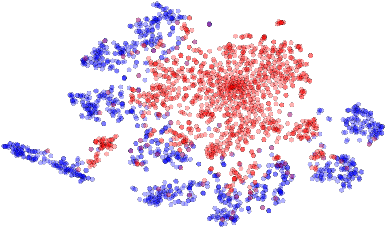
\includegraphics[width=0.45\textwidth]{./figures/adaptation_vis/pool2_mnist2inv_before.pdf}}\hfill%
  \subfigure[Adapted]{%%
    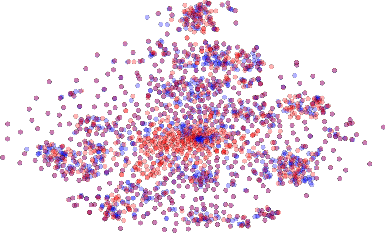
\includegraphics[width=0.45\textwidth]{./figures/adaptation_vis/pool2_mnist2inv_after.pdf}}%%
  \hspace*{\fill}%
  \end{minipage}%
  \begin{minipage}{.5\textwidth}
  \centering
  \small{{\sc Syn Numbers $ \rightarrow $ SVHN}: last hidden layer of the label predictor}
  \setcounter{subfigure}{0}
  \hspace*{\fill}%
  \subfigure[Non-adapted]{%%
    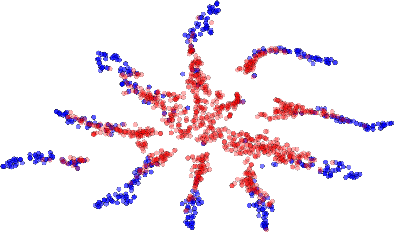
\includegraphics[width=0.45\textwidth]{./figures/adaptation_vis/before.pdf}}\hfill%
  \subfigure[Adapted]{%%
    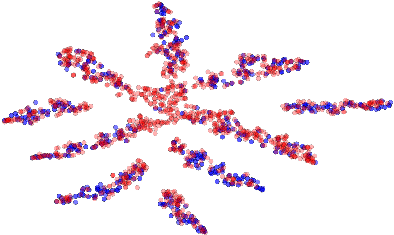
\includegraphics[width=0.45\textwidth]{./figures/adaptation_vis/after.pdf}}%%
  \hspace*{\fill}%
  \end{minipage}
  \caption{The effect of adaptation on the distribution of the extracted features (best viewed in color). The figure shows t-SNE \cite{Maaten13} visualizations of the CNN's activations {\bf (a)} in case when no adaptation was performed and {\bf (b)} in case when our adaptation procedure was incorporated into training. {\it Blue} points correspond to the source domain examples, while {\it red} ones correspond to the target domain. In all cases, the adaptation in our method makes the two distributions of features much closer.}
  \label{fig:exper_adapt_vis}
\end{figure*}

\subsection{Results}
\label{sect:exper_quant}

We now discuss the experimental settings and the results. In each case, we train on the source dataset and test on a different target domain dataset, with considerable shifts between domains (see \fig{exper_domains_examples}). The results are summarized in \tab{results} and \tab{results_office}. 

\vspace{2mm}\noindent {\bf MNIST $ \rightarrow $ MNIST-M.}
Our first experiment deals with the MNIST dataset~\cite{LeCun98} (source). In order to obtain the target domain ({\sc MNIST-M}) we blend digits from the original set over patches randomly extracted from color photos from BSDS500 \cite{Arbelaez11}. This operation is formally defined for two images $ I^{1}, I^{2} $ as $ I_{ijk}^{out} = | I_{ijk}^{1} - I_{ijk}^{2} | $, where $ i, j $ are the coordinates of a pixel and $ k $ is a channel index. In other words, an output sample is produced by taking a patch from a photo and inverting its pixels at positions corresponding to the pixels of a digit. For a human the classification task becomes only slightly harder compared to the original dataset (the digits are still clearly distinguishable) whereas for a CNN trained on MNIST this domain is quite distinct, as the background and the strokes are no longer constant. Consequently, the source-only model performs poorly. Our approach succeeded at aligning feature distributions (\fig{exper_adapt_vis}), which led to successful adaptation results (considering that the adaptation is unsupervised). At the same time, the improvement over source-only model achieved by subspace alignment (SA) \cite{Fernando13} is quite modest, thus highlighting the difficulty of the adaptation task. 

\vspace{2mm}\noindent {\bf Synthetic numbers $ \rightarrow $ SVHN.}
To address a common scenario of training on synthetic data and testing on  real data, we use Street-View House Number dataset {\sc SVHN} \cite{Netzer11} as the target domain and synthetic digits as the source. The latter ({\sc Syn ~Numbers}) consists of ~500,000 images generated by ourselves from Windows fonts by varying the text (that includes different one-, two-, and three-digit numbers), positioning, orientation, background and stroke colors, and the amount of blur. The degrees of variation were chosen manually to simulate SVHN, however the two datasets are still rather distinct, the biggest difference being the structured clutter in the background of SVHN images. 

The proposed backpropagation-based technique works well covering two thirds of the gap between training with source data only and training on target domain data with known target labels. In contrast, SA~\cite{Fernando13} does not result in any significant improvement in the classification accuracy, thus highlighting that the adaptation task is even more challenging than in the case of the MNIST experiment.

\vspace{2mm}\noindent {\bf MNIST $ \leftrightarrow $ SVHN.}
In this experiment, we further increase the gap between distributions, and test on {\sc MNIST} and {\sc SVHN}, which are significantly different in appearance. Training on SVHN even without adaptation is challenging --- classification error stays high during the first 150 epochs. In order to avoid ending up in a poor local minimum we, therefore, do not use learning rate annealing here. Obviously, the two directions ({\sc MNIST} $ \rightarrow $ {\sc SVHN} and {\sc SVHN} $ \rightarrow $ {\sc MNIST}) are not equally difficult. As {\sc SVHN} is more diverse, a model trained on SVHN is expected to be more generic and to perform reasonably on the MNIST dataset. This, indeed, turns out to be the case and is supported by the appearance of the feature distributions. We observe a quite strong separation between the domains when we feed them into the CNN trained solely on { \sc MNIST}, whereas for the {\sc SVHN}-trained network the features are much more intermixed. This difference probably explains why our method succeeded in improving the performance by adaptation in the {\sc SVHN} $ \rightarrow $ {\sc MNIST} scenario (see \tab{results}) but not in the opposite direction (SA is not able to perform adaptation in this case either). Unsupervised adaptation from MNIST to SVHN gives a failure example for our approach (we are unaware of any unsupervised DA methods capable of performing such adaptation).

\vspace{2mm}\noindent {\bf Synthetic Signs $ \rightarrow $ GTSRB.}
Overall, this setting is similar to the {\sc Syn Numbers} $ \rightarrow $ {\sc SVHN} experiment, except the distribution of the features is more complex due to the significantly larger number of classes (43 instead of 10). For the source domain we obtained~100,000 synthetic images (which we call {\sc Syn~Signs}) simulating various photoshooting conditions. Once again, our method achieves a sensible increase in performance once again proving its suitability for the synthetic-to-real data adaptation.

\begin{figure}
  \centering
  \setlength\figureheight{2.7cm}
  \setlength\figurewidth{6.8cm}
  % This file was created by matlab2tikz v0.5.0 running on MATLAB 8.3.
%Copyright (c) 2008--2014, Nico Schlömer <nico.schloemer@gmail.com>
%All rights reserved.
%Minimal pgfplots version: 1.3
%
%The latest updates can be retrieved from
%  http://www.mathworks.com/matlabcentral/fileexchange/22022-matlab2tikz
%where you can also make suggestions and rate matlab2tikz.
%
\begin{tikzpicture}[font=\scriptsize]

\begin{axis}[%
width=0.95092\figurewidth,
height=\figureheight,
at={(0\figurewidth,0\figureheight)},
scale only axis,
xmin=10000,
xmax=50000,
xlabel={Batches seen},
ymin=0,
ymax=1,
ylabel={Validation error},
axis x line*=bottom,
axis y line*=left,
legend style={at={($ (1,1) + (-0.1cm,-0.1cm) $)},anchor=north east,align=left,legend cell align=left,draw=black},
xmajorgrids,
ymajorgrids,
grid style={dashed}
]
\addplot [color=blue,solid,line width=1.0pt]
  table[row sep=crcr]{%
10500	0.199757996632997\\
11000	0.19162984006734\\
11500	0.190788089225589\\
12000	0.192918771043771\\
12500	0.196390993265993\\
13000	0.185527146464646\\
13500	0.190472432659933\\
14000	0.185606060606061\\
14500	0.183422769360269\\
15000	0.189051978114478\\
15500	0.191524621212121\\
16000	0.186079545454545\\
16500	0.179424452861953\\
17000	0.187684132996633\\
17500	0.187868265993266\\
18000	0.180923821548822\\
18500	0.187315867003367\\
19000	0.178661616161616\\
19500	0.18102904040404\\
20000	0.180555555555556\\
20500	0.176662457912458\\
21000	0.183791035353535\\
21500	0.179214015151515\\
22000	0.178898358585859\\
22500	0.178898358585859\\
23000	0.174479166666667\\
23500	0.174742213804714\\
24000	0.171059553872054\\
24500	0.177951388888889\\
25000	0.174794823232323\\
25500	0.174084595959596\\
26000	0.174636994949495\\
26500	0.169034090909091\\
27000	0.171191077441077\\
27500	0.170875420875421\\
28000	0.171506734006734\\
28500	0.170217803030303\\
29000	0.169244528619529\\
29500	0.169875841750842\\
30000	0.168744739057239\\
30500	0.17048085016835\\
31000	0.169454966329966\\
31500	0.167771464646465\\
32000	0.168849957912458\\
32500	0.168323863636364\\
33000	0.168718434343434\\
33500	0.165667087542088\\
34000	0.167376893939394\\
34500	0.169007786195286\\
35000	0.167140151515152\\
35500	0.165667087542088\\
36000	0.167850378787879\\
36500	0.169823232323232\\
37000	0.170691287878788\\
37500	0.16640361952862\\
38000	0.167981902356902\\
38500	0.169875841750842\\
39000	0.166771885521886\\
39500	0.169376052188552\\
40000	0.168087121212121\\
40500	0.165509259259259\\
41000	0.167718855218855\\
41500	0.168060816498317\\
42000	0.166035353535354\\
42500	0.166692971380471\\
43000	0.166429924242424\\
43500	0.167034932659933\\
44000	0.170349326599327\\
44500	0.169744318181818\\
45000	0.168218644781145\\
45500	0.166429924242424\\
46000	0.166324705387205\\
46500	0.168771043771044\\
47000	0.168034511784512\\
47500	0.168718434343434\\
48000	0.171059553872054\\
48500	0.170638678451178\\
49000	0.16819234006734\\
49500	0.168981481481481\\
50000	0.167902988215488\\
};
\addlegendentry{Real data only};

\addplot [color=cyan,solid,line width=1.0pt]
  table[row sep=crcr]{%
10500	0.9625\\
11000	0.79765625\\
11500	0.715625\\
12000	0.6140625\\
12500	0.52109375\\
13000	0.459375\\
13500	0.4484375\\
14000	0.421875\\
14500	0.39453125\\
15000	0.4109375\\
15500	0.34296875\\
16000	0.36875\\
16500	0.3359375\\
17000	0.36171875\\
17500	0.3171875\\
18000	0.3484375\\
18500	0.32421875\\
19000	0.315625\\
19500	0.346875\\
20000	0.31875\\
20500	0.35390625\\
21000	0.3265625\\
21500	0.33359375\\
22000	0.3171875\\
22500	0.28515625\\
23000	0.30546875\\
23500	0.309375\\
24000	0.2796875\\
24500	0.30859375\\
25000	0.30703125\\
25500	0.3078125\\
26000	0.28671875\\
26500	0.2875\\
27000	0.31484375\\
27500	0.2859375\\
28000	0.29375\\
28500	0.31328125\\
29000	0.3078125\\
29500	0.2859375\\
30000	0.2890625\\
30500	0.284375\\
31000	0.2953125\\
31500	0.26953125\\
32000	0.29921875\\
32500	0.30078125\\
33000	0.2640625\\
33500	0.309375\\
34000	0.2734375\\
34500	0.290625\\
35000	0.26796875\\
35500	0.3015625\\
36000	0.26796875\\
36500	0.2921875\\
37000	0.265625\\
37500	0.2765625\\
38000	0.2859375\\
38500	0.32109375\\
39000	0.28046875\\
39500	0.275\\
40000	0.24921875\\
40500	0.29140625\\
41000	0.26640625\\
41500	0.265625\\
42000	0.259375\\
42500	0.2765625\\
43000	0.26796875\\
43500	0.2765625\\
44000	0.27265625\\
44500	0.25546875\\
45000	0.26484375\\
45500	0.271875\\
46000	0.2703125\\
46500	0.26171875\\
47000	0.246875\\
47500	0.25078125\\
48000	0.29609375\\
48500	0.2640625\\
49000	0.26875\\
49500	0.26015625\\
50000	0.2578125\\
};
\addlegendentry{Synthetic data only};

\addplot [color=red,solid,line width=1.0pt]
  table[row sep=crcr]{%
10500	0.943892045454545\\
11000	0.943892045454545\\
11500	0.943892045454545\\
12000	0.943892045454545\\
12500	0.848300715488216\\
13000	0.658722643097643\\
13500	0.590593434343434\\
14000	0.475484006734007\\
14500	0.313946759259259\\
15000	0.235690235690236\\
15500	0.17879313973064\\
16000	0.152383207070707\\
16500	0.12912984006734\\
17000	0.114478114478114\\
17500	0.116214225589226\\
18000	0.1015625\\
18500	0.10066813973064\\
19000	0.101983375420875\\
19500	0.0914351851851852\\
20000	0.0895675505050505\\
20500	0.0894360269360269\\
21000	0.0827283249158249\\
21500	0.0798611111111111\\
22000	0.0859638047138047\\
22500	0.0799137205387205\\
23000	0.0778619528619529\\
23500	0.0737584175084175\\
24000	0.0742582070707071\\
24500	0.0776778198653199\\
25000	0.0771517255892256\\
25500	0.0725747053872054\\
26000	0.0739425505050505\\
26500	0.0734953703703704\\
27000	0.0730744949494949\\
27500	0.0688920454545455\\
28000	0.0702072811447811\\
28500	0.072337962962963\\
29000	0.0670244107744108\\
29500	0.0733638468013468\\
30000	0.0667613636363636\\
30500	0.0692340067340067\\
31000	0.0652093855218855\\
31500	0.0664720117845118\\
32000	0.0655776515151515\\
32500	0.0671296296296296\\
33000	0.0656039562289562\\
33500	0.0646043771043771\\
34000	0.0668665824915825\\
34500	0.0638678451178451\\
35000	0.065077861952862\\
35500	0.0649989478114478\\
36000	0.0672348484848485\\
36500	0.0668665824915825\\
37000	0.0626052188552189\\
37500	0.0652093855218855\\
38000	0.0626315235690236\\
38500	0.0627893518518518\\
39000	0.0613162878787879\\
39500	0.063236531986532\\
40000	0.0629208754208754\\
40500	0.0639467592592593\\
41000	0.0612899831649832\\
41500	0.0653409090909091\\
42000	0.0608691077441077\\
42500	0.0613425925925926\\
43000	0.0630260942760943\\
43500	0.060106271043771\\
44000	0.0638678451178451\\
44500	0.0602377946127946\\
45000	0.0577388468013468\\
45500	0.062684132996633\\
46000	0.0608164983164983\\
46500	0.0603167087542088\\
47000	0.0577651515151515\\
47500	0.0583175505050505\\
48000	0.0591329966329966\\
48500	0.0607112794612795\\
49000	0.0585805976430976\\
49500	0.0583175505050505\\
50000	0.0590540824915825\\
};
\addlegendentry{Both};

\end{axis}
\end{tikzpicture}%
  \caption{Semi-supervised domain adaptation for the traffic signs. As labeled target domain data are shown to the method, it achieves significantly lower error than the model trained on target domain data only or on source domain data only. \vspace{-4mm}}
  \label{fig:exper_semi_test}
\end{figure}

As an additional experiment, we also evaluate the proposed algorithm for semi-supervised domain adaptation, i.e.\ when one is additionally provided with a small amount of labeled target data. For that purpose we split {\sc GTSRB} into the train set (1280 random samples with labels) and the validation set (the rest of the dataset). The validation part is used solely for the evaluation and does not participate in the adaptation. The training procedure changes slightly as the label predictor is now exposed to the target data. \fig{exper_semi_test} shows the change of the validation error throughout the training. While the graph clearly suggests that our method can be used in the semi-supervised setting, thorough verification of semi-supervised setting is left for future work.


\vspace{2mm}\noindent {\bf Office dataset.} 
We finally evaluate our method on {\sc Office} dataset, which is a collection of three distinct domains: {\sc Amazon}, {\sc DSLR}, and {\sc Webcam}. Unlike previously discussed datasets, {\sc Office} is rather small-scale with only 2817 labeled images spread across 31 different categories in the largest domain. The amount of available data is crucial for a successful training of a deep model, hence we opted for the fine-tuning of the CNN pre-trained on the ImageNet \cite{Jia14} as it is done in some recent DA works \cite{Donahue14,Tzeng14,Hoffman14}. We make our approach more comparable with \cite{Tzeng14} by using exactly the same network architecture replacing domain mean-based regularization with the domain classifier.

Following most previous works, we evaluate our method using 5 random splits for each of the 3 transfer tasks commonly used for evaluation. Our training protocol is close to \cite{Tzeng14,Saenko10,Gong12} as we use the same number of labeled source-domain images per category. Unlike those works and similarly to e.g.\ DLID~\cite{Chopra13} we use the whole unlabeled target domain (as the premise of our method is the abundance of unlabeled data in the target domain). Under this transductive setting, our method is able to improve previously-reported state-of-the-art accuracy for unsupervised adaptation very considerably (\tab{results_office}), especially in the most challenging {\sc Amazon} $ \rightarrow $ {\sc Webcam} scenario (the two domains with the largest domain shift).

\section{Discussion}
\label{sec:discussion}

The accuracy on the CKP set shows that the chosen approach is robust, misclassification usually occurs on pictures which are the first few instances of an emotion sequence. Often a neutral facial expression is depicted in those frames. Thus those misclassifications are not necessarily an error in the approach, but in the data selection. Other than that no major problem could be detected. The emotion \textit{Surprise} is often confused with \textit{Disgust} with a rate of 0.045\% which is the highest. Of those images, where an emotion is present, only few are wrongly classified.\\ 


As there is no consent for the misclassified images, they cannot be depicted here. However some unique names are provided. \\
Image S119\_001\_00000010 is classified as \textit{Fear} while the annotated emotion corresponds to \textit{Surprise}. The image depicts a person with a wide open mouth and open eyes. Pictures representing \textit{Surprise} are often very similar, since the persons also have wide open mouths and eyes. In image S032\_004\_00000014 the targeted label \textit{Fear} is confused with \textit{Anger}. While the mouth region in pictures with \textit{Anger} differ, the eye regions are alike, since in both situations the eyes and eyebrows are contracted.\\
Similar effects are experienced when dealing with the MMI Dataset. Since the first two frames are discarded most pictures with neutral positions are excluded. In few images a neutral position can still be found which gives rise to errors. For the same reason as the CKP set images will not be displayed. Due to the approach to extract images of the videos, a unique identifier for the misclassified image cannot be provided.\\
The top confusions are observed for \textit{Fear} and \textit{Surprise} with a rate of 0.0159\% where \textit{Fear} is wrongly misclassified as \textit{Surprise}. Session 1937 shows a woman displaying \textit{Fear} but it is classified as \textit{Surprise}. Both share common features like similar eye and mouth movement. In both emotions, participants move the head slightly backwards. This can be identified by wrinkled skin. The second most confusion rate, \textit{Surprise} being mistaken as \textit{Sadness}, is mostly based on neutral position images. Although the first two images are not used, some selected frames still do not contain an emotion. In Session 1985 \textit{Surprise} is being mistaken as \textit{Sadness}. The image depicts a man with his mouth being slightly curved, making him look sad.\\

DeXpression extracts features and uses them to classify images, but in very few cases the emotions are confused. This happens, as discussed, usually in pictures depicting no emotion. DeXpression performs very well on both tested sets, if an emotion is present.



\appendix
\renewcommand\thesection{Appendix \Alph{section}}
\newcommand{\vv}[1]{{\texttt{#1}}}
\newcommand{\conv}{\vv{conv}}
\newcommand{\fc}{\vv{fc}}
\newcolumntype{x}{>\small c}

\newcommand{\trainval}{trainval\raisebox{0.2ex}{$\ast$}}
\newcolumntype{L}[1]{>{\raggedright\let\newline\\\arraybackslash\hspace{0pt}}m{#1}}
\newcolumntype{C}[1]{>{\centering\let\newline\\\arraybackslash\hspace{0pt}}m{#1}}
\newcolumntype{R}[1]{>{\raggedleft\let\newline\\\arraybackslash\hspace{0pt}}m{#1}}
\newcommand{\hl}[1]{\underline{\textbf{#1}}}
\newcolumntype{o}{>\small L}
% \renewcommand{\baselinestretch}{0.99}

\clearpage
\onecolumn

% \commentAS{Discuss making the text regular size.}\\
% \commentAS{Standardize table sizes and format.}

\section*{Appendix A}

\subsubsection*{De-duplication Experiments}
A dataset with 300M images is almost guaranteed to contain images that overlap with the validation set of target tasks. In fact, we find that even for ImageNet, there are 890 out of 50K validation images have near-duplicate images in the training.

We use visual embeddings to measure similarities and identify duplicate or near-duplicate images. The embeddings are based on deep learning features. We find there are 5536 out of 50K images in ImageNet validation set, 1648 out of 8K images in COCO \minival, 201 out of 4952 images in Pascal VOC 2007 test set, and 84 out of 1449 images in Pascal VOC 2012 validation set that have near duplicates in JFT-300M. We rerun several experiments by removing near-duplicate images from validation sets and then comparing performance between baselines and learned models. We observe no significant differences in trends. Table~\ref{tab:imagenet_dedup},~\ref{tab:coco_dedup} and ~\ref{tab:pascal_dedup} show that the duplicate images have minimal impact on performance for all experiments.

\begin{table*}[h]
\centering
\renewcommand{\arraystretch}{1.1}
\renewcommand{\tabcolsep}{1.2mm}
% \resizebox{0.7\linewidth}{!}{
\begin{tabular}{@{} l | c  c | c  c @{}}
& \multicolumn{2}{c|}{Original} & \multicolumn{2}{c}{De-duplication} \\
& Top-1 Acc. & Top-5 Acc. & Top-1 Acc. & Top-5 Acc. \\
\hline
MSRA checkpoint & 76.4 & 92.9 & 76.4 & 92.9 \\
Random initialization & 77.5 & 93.9 & 77.5 & 93.8 \\
Fine-tune from JFT-300M & 79.2 & 94.7 & 79.3 & 94.7 \\
\end{tabular}
% }
\vspace{0.05in}
\caption{Top-1 and top-5 classification accuracy on ImageNet validation set, before and after de-duplication. Single model and single crop are used.}
\label{tab:imagenet_dedup}
\end{table*}
\vspace{-0.1in}

\begin{table*}[h]
\centering
\renewcommand{\arraystretch}{1.1}
\renewcommand{\tabcolsep}{1.2mm}
% \resizebox{0.7\linewidth}{!}{
\begin{tabular}{@{} l | c  c | c  c @{}}
& \multicolumn{2}{c|}{Original} & \multicolumn{2}{c}{De-duplication} \\
& mAP@0.5 & mAP@[0.5,0.95] & mAP@0.5 & mAP@[0.5,0.95] \\
\hline
ImageNet & 54.0 & 34.5 & 54.0 & 34.6 \\
300M & 57.1 & 36.8 & 56.8 & 36.7 \\
ImageNet+300M & 58.2 & 37.8 & 58.2 & 37.7 \\
\end{tabular}
% }
\vspace{0.07in}
\caption{mAP@0.5 and mAP@[0.5,0.95] for object detection performance on COCO \minival, before and after de-duplication.}
\label{tab:coco_dedup}
\end{table*}
\vspace{-0.1in}

\begin{table*}[h]
\centering
\renewcommand{\arraystretch}{1.1}
\renewcommand{\tabcolsep}{1.2mm}
% \resizebox{0.7\linewidth}{!}{
\begin{tabular}{@{} l | c  c | c  c @{}}
& \multicolumn{2}{c|}{VOC07 Detection} & \multicolumn{2}{c}{VOC12 Segmentation} \\
& Original & De-duplication & Original & De-duplication \\
\hline
ImageNet & 76.3 & 76.5 & 73.6 & 73.3 \\
300M & 81.4 & 81.5 & 75.3 & 75.1 \\
ImageNet+300M & 81.3 & 81.2 & 76.5 & 76.5 \\
\end{tabular}
% }
\vspace{0.05in}
\caption{Object detection and semantic segmentation performance on Pascal VOC, before and after deduplication. (Left) Object detection mAP@0.5 on Pascal VOC 2007 test set. (Right) Semantic segmentation mIOU on Pascal VOC 2012 validation set.}
\label{tab:pascal_dedup}
\end{table*}

We do not conduct de-duplication experiments of COCO testdev dataset for object detection and pose estimation as their groundtruth annotations are not publicly available.


\clearpage

\section*{Appendix B}

\subsubsection*{Detailed and Per-category Results: Object Detection}
In this section, we present detailed and per-category object detection results for Table 2 (Section 5.2) from the main submission, evaluated on the COCO test-dev split. In Table~\ref{tab:coco_main}, we report detailed AP and AR results using different initializations. In Table~\ref{tab:per_category}, we provide per-category AP and AP@.5 results.  


\begin{table*}[h]
\centering
\renewcommand{\arraystretch}{1.1}
\renewcommand{\tabcolsep}{1.2mm}
% \resizebox{\linewidth}{!}{
\begin{tabular}{@{} l | c  c  c  c  c  c | c  c  c  c  c  c @{}}

& AP & AP@.5 & AP@.75 & AP(S) & AP(M) & AP(L) & AR & AR@.5 & AR@.75 & AR(S) & AR(M) & AR(L)\\
\hline
ImageNet & 34.3 & 53.6 & 36.9 & 15.1 & 37.4 & 48.5 & 30.2 & 47.3 & 49.7 & 26.0 & 54.6 & 68.6\\
300M & 36.7 & 56.9 & 39.5 & 17.1 & 40.0 & 50.7 & 31.5 & 49.3 & 51.9 & 28.6 & 56.9 & 70.4 \\
ImageNet+300M & 37.4 & 58.0 & 40.1 & 17.5 & 41.1 & 51.2 & 31.8 & 49.8 & 52.4 & 29.0 & 57.7 & 70.5 \\
\end{tabular}
% }
\vspace{0.1in}
\caption{Object detection performance on COCO test-dev split using different model initializations.}
\label{tab:coco_main}
\end{table*}
\vspace{-0.1in}

\subsubsection*{Per-category Results: Semantic Segmentation}
In Table~\ref{tab:segmentation_supp}, we report quantitative results on the VOC 2012 segmentation validation set for all classes (refer to Figure 5 (left), Section 5.3 in the main submission). Results are reported for different initializations. We observe more than 7 point improvement for categories like boat and horse.


\begin{table*}[h]
	\centering
	\renewcommand{\arraystretch}{1.1}
	\renewcommand{\tabcolsep}{1.2mm}
	\resizebox{\linewidth}{!}{
		\begin{tabular}{@{}L{2.5cm} c c*{29}{x} @{}}
			\toprule
			Initialization & mIOU & bg & {aero} & {bike} & {bird} & {boat} & {bottle} & {bus} & {car}& {cat} & {chair} & {cow} & {table} & {dog} & {horse} & {mbike} & {persn} & {plant} & {sheep} & {sofa} & {train} & {tv} \\
			\midrule
			ImageNet &
			73.6 & 93.2 & 88.9 & 40.1 & 87.3 & 65.0 & 78.8 & 89.9 & 84.3 & 88.8 & 37.2 & 81.6 & 49.3 & 84.1 & 78.9 & 79.3 & 83.3 & 57.7 & 82.0 & 41.7 & 80.3 & 73.1 \\
			300M &
			75.3 & 93.7 & 89.8 & 40.1 & 89.8 & 70.6 & 78.5 & 89.9 & 86.1 & 92.0 & 36.9 & 80.9 & 52.8 & 87.6 & 82.4 & 80.8 & 84.3 & 61.7 & 84.4 & 44.8 & 80.9 & 72.6\\
			ImageNet+300M &
			76.5 & 94.8 & 90.4 & 41.6 & 89.1 & 73.1 & 80.4 & 92.3 & 86.7 & 92.0 & 39.6 & 82.7 & 52.7 & 86.2 & 86.1 & 83.6 & 85.7 & 61.5 & 83.9 & 45.3 & 84.6 & 73.6 \\
			\bottomrule
		\end{tabular}
	}
	\vspace{0.01in}
	\caption{Per-class semantic segmentation performance on PASCAL VOC 2012 validation set.}
	\label{tab:segmentation_supp}
\end{table*}
\vspace{-0.1in}

\subsubsection*{Detailed Results: Human Pose Estimation}
In Table~\ref{tab:coco_pose_supp}, we present all AP and AR results for the performance reported in Table 7 (Section 5.4) in the main submission.
%Please note that we reported incorrect baseline AR and AR@.5 performance for ImageNet baseline in the main submission (the performance is 66.7 AR and 86.6 AR@.5 instead of 68.6 and 88.1 respectively as reported in Table 7, Section 5.4).

% \vspace{-0.1in}
\begin{table*}[h]
\centering
\begin{tabular}{@{} l | c  c  c  c  c | c  c  c  c  c @{}}
& AP & AP@.5 & AP@.75 & AP(M) & AP(L) & AR & AR@.5 & AR@.75 & AR(M) & AR(L)\\
\hline
CMU Pose~[3] & 61.8 & 84.9 & 67.5 & 57.1 & 68.2 & 66.5 & 87.2 & 71.8 & 60.6 & 74.6 \\
ImageNet~[26] & 62.4 & 84.0 & 68.5 & 59.1 & 68.1 & 66.7 & 86.6 & 72.0 & 60.8 & 74.9\\
300M & 64.8 & 85.8 & 71.5 & 62.2 & 70.3 & 69.4 & 88.4 & 75.2 & 63.9 & 77.0\\
ImageNet+300M & 64.4 & 85.7 & 70.7 & 61.8 & 69.8 & 69.1 & 88.2 & 74.8 & 63.7 & 76.6\\
\end{tabular}
\vspace{0.05in}
\caption{Human pose estimation performance on the COCO test-dev split.}
\label{tab:coco_pose_supp}
\end{table*}


\begin{table*}[h!]
\centering
\caption{Per-class object detection performance on COCO test-dev split using different model initializations.}
\label{tab:allclasses}
\vspace{0.1in}
\renewcommand{\arraystretch}{1.2}
\renewcommand{\tabcolsep}{1.2mm}
\resizebox{0.485\linewidth}{!}{
\footnotesize
\begin{tabular}{@{}
L{1.7cm} 
!{\color{gray}\vrule} cc
!{\color{gray}\vrule} cc
!{\color{gray}\vrule} cc
@{}}
\Xhline{1pt}
\multicolumn{1}{r!{\color{gray}\vrule}}{Initialization $\rightarrow$} & \multicolumn{2}{c!{\color{gray}\vrule}}{ImageNet} & \multicolumn{2}{c!{\color{gray}\vrule}}{300M} &
\multicolumn{2}{c}{{\footnotesize ImageNet+300M}}\\
& \scriptsize AP@.5 & \scriptsize AP &  \scriptsize AP@.5 & \scriptsize AP & \scriptsize AP@.5 & \scriptsize AP \\ 
\Xhline{0.5pt}
person & 71.5 & 47.7 & 73.1 & 49.8 & 72.7 & 49.9 \\
bicycle & 48.9 & 26.4 & 54.9 & 30.0 & 52.7 & 29.9 \\
car & 55.7 & 34.7 & 58.3 & 36.9 & 59.3 & 37.1 \\
motorcycle & 56.5 & 36.7 & 61.6 & 40.5 & 59.9 & 39.6 \\
airplane & 67.9 & 52.0 & 70.1 & 55.0 & 70.4 & 54.7 \\
bus & 77.7 & 62.5 & 79.5 & 64.6 & 79.0 & 64.2 \\
train & 66.8 & 59.2 & 69.7 & 62.8 & 69.7 & 62.1 \\
truck & 46.3 & 29.9 & 49.7 & 33.0 & 52.2 & 34.5 \\
boat & 30.6 & 19.4 & 32.5 & 22.1 & 32.1 & 22.3 \\
traffic light & 48.9 & 22.7 & 49.8 & 24.3 & 49.1 & 24.6 \\
fire hydrant & 75.3 & 59.1 & 74.4 & 59.3 & 74.9 & 59.5 \\
stop sign & 83.2 & 63.6 & 84.4 & 63.8 & 85.6 & 66.4 \\
parking meter & 62.2 & 37.5 & 64.9 & 38.5 & 64.5 & 37.6 \\
bench & 38.1 & 19.6 & 39.3 & 20.1 & 40.6 & 21.4 \\
bird & 60.2 & 29.4 & 61.9 & 33.0 & 63.3 & 34.2 \\
cat & 64.2 & 58.1 & 68.0 & 61.9 & 67.9 & 62.4 \\
dog & 62.6 & 52.9 & 66.1 & 56.2 & 66.9 & 57.3 \\
horse & 67.2 & 53.5 & 70.8 & 57.0 & 71.3 & 57.0 \\
sheep & 64.4 & 43.6 & 64.8 & 45.4 & 66.7 & 46.3 \\
cow & 70.7 & 45.4 & 71.9 & 47.4 & 73.3 & 48.9 \\
elephant & 75.1 & 64.1 & 77.3 & 66.4 & 76.1 & 65.5 \\
bear & 70.5 & 66.9 & 74.5 & 69.8 & 72.7 & 70.0 \\
zebra & 71.0 & 59.3 & 71.5 & 60.4 & 71.3 & 61.0 \\
giraffe & 75.3 & 67.4 & 75.9 & 69.0 & 75.9 & 69.3 \\
backpack & 19.6 & 12.8 & 19.5 & 14.7 & 18.5 & 15.1 \\
umbrella & 46.2 & 28.9 & 50.7 & 32.3 & 50.4 & 32.8 \\
handbag & 14.7 & 9.7 & 13.7 & 10.9 & 16.1 & 12.0 \\
tie & 50.8 & 26.3 & 53.2 & 27.9 & 51.5 & 28.4 \\
suitcase & 40.4 & 26.7 & 44.4 & 30.3 & 46.9 & 32.5 \\
frisbee & 53.4 & 43.8 & 55.3 & 48.6 & 58.6 & 48.3 \\
skis & 1.5 & 18.1 & 3.0 & 20.0 & 2.3 & 20.7 \\
snowboard & 45.7 & 29.3 & 47.0 & 33.3 & 43.9 & 32.1 \\
sports ball & 41.8 & 35.6 & 48.7 & 37.6 & 42.3 & 38.6 \\
kite & 39.4 & 37.5 & 33.9 & 38.9 & 35.9 & 40.0 \\
baseball bat & 8.3 & 23.4 & 6.7 & 25.1 & 9.9 & 27.5 \\
baseball glove & 35.6 & 27.4 & 33.7 & 31.2 & 41.9 & 31.8 \\
skateboard & 42.2 & 40.0 & 48.6 & 44.7 & 49.2 & 44.4 \\
surfboard & 48.5 & 31.1 & 51.7 & 32.8 & 52.4 & 33.9 \\
tennis racket & 53.1 & 42.6 & 55.1 & 44.1 & 55.4 & 45.1 \\
bottle & 61.2 & 28.6 & 61.8 & 30.5 & 61.6 & 30.8 \\
\Xhline{1pt}
\end{tabular}
}
\hspace{0.2cm}
\resizebox{0.485\linewidth}{!}{
\footnotesize
\begin{tabular}{@{}
L{1.7cm} 
!{\color{gray}\vrule} cc
!{\color{gray}\vrule} cc
!{\color{gray}\vrule} cc
@{}}
\Xhline{1pt}
\multicolumn{1}{r!{\color{gray}\vrule}}{Initialization $\rightarrow$} & \multicolumn{2}{c!{\color{gray}\vrule}}{ImageNet} & \multicolumn{2}{c!{\color{gray}\vrule}}{300M} &
\multicolumn{2}{c}{{\footnotesize ImageNet+300M}}\\
& \scriptsize AP@.5 & \scriptsize AP &  \scriptsize AP@.5 & \scriptsize AP & \scriptsize AP@.5 & \scriptsize AP \\ 
\Xhline{0.5pt}
wine glass & 53.8 & 30.2 & 56.3 & 33.3 & 58.7 & 34.7 \\
cup & 64.7 & 32.5 & 67.5 & 35.6 & 68.4 & 35.9 \\
fork & 45.7 & 23.2 & 45.1 & 26.5 & 50.1 & 27.8 \\
knife & 29.9 & 12.8 & 37.1 & 15.7 & 37.2 & 16.4 \\
spoon & 13.0 & 10.0 & 11.4 & 11.7 & 11.6 & 13.3 \\
bowl & 49.4 & 32.1 & 53.6 & 35.4 & 52.2 & 35.4 \\
banana & 38.1 & 18.7 & 39.8 & 20.4 & 40.0 & 21.1 \\
apple & 49.4 & 19.1 & 50.1 & 20.8 & 51.5 & 21.7 \\
sandwich & 44.0 & 29.6 & 45.2 & 31.3 & 47.8 & 34.1 \\
orange & 48.7 & 25.0 & 50.7 & 26.2 & 49.0 & 26.1 \\
broccoli & 30.6 & 22.9 & 32.5 & 24.8 & 31.9 & 24.6 \\
carrot & 25.9 & 14.0 & 28.6 & 16.1 & 21.5 & 16.4 \\
hot dog & 43.7 & 21.8 & 46.5 & 24.8 & 48.2 & 25.8 \\
pizza & 67.9 & 51.1 & 69.0 & 52.3 & 68.7 & 52.8 \\
donut & 60.2 & 40.1 & 64.8 & 43.9 & 66.8 & 46.4 \\
cake & 42.7 & 25.5 & 46.4 & 28.1 & 46.5 & 29.1 \\
chair & 33.0 & 21.1 & 36.7 & 24.0 & 35.9 & 24.4 \\
couch & 41.3 & 36.2 & 44.5 & 38.9 & 44.9 & 39.4 \\
potted plant & 25.6 & 20.1 & 27.3 & 21.9 & 30.0 & 23.4 \\
bed & 44.5 & 40.6 & 45.6 & 41.7 & 47.2 & 43.4 \\
dining table & 33.9 & 25.3 & 36.3 & 27.5 & 36.8 & 27.6 \\
toilet & 61.1 & 54.8 & 61.8 & 56.1 & 63.3 & 57.4 \\
tv & 61.8 & 50.0 & 63.0 & 51.9 & 63.7 & 52.7 \\
laptop & 65.8 & 54.5 & 68.3 & 56.6 & 68.9 & 57.5 \\
mouse & 72.1 & 44.4 & 72.0 & 47.6 & 75.6 & 47.3 \\
remote & 56.4 & 22.1 & 55.8 & 24.4 & 59.1 & 26.0 \\
keyboard & 57.1 & 45.4 & 57.5 & 45.9 & 61.4 & 48.3 \\
cell phone & 54.0 & 23.4 & 58.5 & 26.1 & 57.5 & 26.7 \\
microwave & 53.9 & 50.3 & 53.7 & 50.5 & 58.7 & 53.1 \\
oven & 40.9 & 31.7 & 41.9 & 33.5 & 43.2 & 34.6 \\
toaster & 32.6 & 14.7 & 39.9 & 20.5 & 32.9 & 20.1 \\
sink & 43.2 & 31.0 & 44.8 & 34.4 & 44.0 & 33.9 \\
refrigerator & 48.6 & 42.3 & 51.7 & 44.6 & 52.4 & 46.1 \\
book & 15.2 & 7.4 & 18.7 & 8.8 & 21.3 & 9.8 \\
clock & 56.7 & 43.7 & 56.7 & 45.3 & 55.8 & 45.1 \\
vase & 57.1 & 32.3 & 61.5 & 35.9 & 61.4 & 36.5 \\
scissors & 31.1 & 20.8 & 38.9 & 25.2 & 34.8 & 25.9 \\
teddy bear & 50.4 & 35.4 & 54.7 & 40.2 & 54.7 & 40.4 \\
hair drier & 2.3 & 1.0 & 4.8 & 1.8 & 4.0 & 1.9 \\
toothbrush & 48.5 & 34.3 & 50.7 & 36.7 & 51.2 & 37.4 \\
\Xhline{1pt}
\end{tabular}
}
\label{tab:per_category}
\end{table*}


\newpage
\bibliography{paper}
\bibliographystyle{icml2015}

\end{document} 


% This document was modified from the file originally made available by
% Pat Langley and Andrea Danyluk for ICML-2K. This version was
% created by Lise Getoor and Tobias Scheffer, it was slightly modified  
% from the 2010 version by Thorsten Joachims & Johannes Fuernkranz, 
% slightly modified from the 2009 version by Kiri Wagstaff and 
% Sam Roweis's 2008 version, which is slightly modified from 
% Prasad Tadepalli's 2007 version which is a lightly 
% changed version of the previous year's version by Andrew Moore, 
% which was in turn edited from those of Kristian Kersting and 
% Codrina Lauth. Alex Smola contributed to the algorithmic style files.  
